%% AI Open (KeAi) manuscript, official Elsevier CAS single-column template (cas-sc).
\documentclass[a4paper,fleqn]{cas-sc}
\usepackage[authoryear]{natbib}
\usepackage{amsmath,amssymb}
\usepackage{booktabs,multirow,graphicx,xcolor}
\usepackage[ruled,vlined,linesnumbered]{algorithm2e}

\newtheorem{proposition}{Proposition}
\newtheorem{corollary}{Corollary}
\newdefinition{remark}{Remark}
\newproof{pf}{Proof}

\newcommand{\ppr}{\mathrm{PPR}}
\newcommand{\repourl}{https://github.com/Akramtaha98/twohop-graph-rerank-rag}
\IfFileExists{tables/numbers.tex}{\newcommand{\nQHotpotQA}{1000}
\newcommand{\nPHotpotQA}{9760}
\newcommand{\RHotpotQANoneRecall}{0.0}
\newcommand{\RHotpotQANoneAllSupp}{0.0}
\newcommand{\RHotpotQANoneEM}{13.3}
\newcommand{\RHotpotQANoneFOne}{18.9}
\newcommand{\RHotpotQANoneSupport}{0.0}
\newcommand{\RHotpotQANoneUnsupp}{100.0}
\newcommand{\RHotpotQANoneSec}{145.8}
\newcommand{\RHotpotQABmTwoRecall}{73.8}
\newcommand{\RHotpotQABmTwoAllSupp}{51.3}
\newcommand{\RHotpotQABmTwoEM}{33.8}
\newcommand{\RHotpotQABmTwoFOne}{42.8}
\newcommand{\RHotpotQABmTwoSupport}{87.1}
\newcommand{\RHotpotQABmTwoUnsupp}{13.4}
\newcommand{\RHotpotQABmTwoSec}{491.7}
\newcommand{\RHotpotQADenseRecall}{84.3}
\newcommand{\RHotpotQADenseAllSupp}{70.2}
\newcommand{\RHotpotQADenseEM}{37.5}
\newcommand{\RHotpotQADenseFOne}{47.6}
\newcommand{\RHotpotQADenseSupport}{88.7}
\newcommand{\RHotpotQADenseUnsupp}{11.9}
\newcommand{\RHotpotQADenseSec}{504.8}
\newcommand{\RHotpotQAGraphRecall}{49.0}
\newcommand{\RHotpotQAGraphAllSupp}{23.4}
\newcommand{\RHotpotQAGraphSec}{9.2}
\newcommand{\RHotpotQAHybridRecall}{84.3}
\newcommand{\RHotpotQAHybridAllSupp}{70.1}
\newcommand{\RHotpotQAHybridEM}{36.6}
\newcommand{\RHotpotQAHybridFOne}{46.8}
\newcommand{\RHotpotQAHybridSupport}{88.2}
\newcommand{\RHotpotQAHybridUnsupp}{12.3}
\newcommand{\RHotpotQAHybridSec}{575.6}
\newcommand{\RHotpotQAAblNoEntitySeedRecall}{84.7}
\newcommand{\RHotpotQAAblNoEntitySeedAllSupp}{71.0}
\newcommand{\RHotpotQAAblNoEntitySeedSec}{19.6}
\newcommand{\RHotpotQAAblNoDenseSeedRecall}{69.0}
\newcommand{\RHotpotQAAblNoDenseSeedAllSupp}{47.2}
\newcommand{\RHotpotQAAblNoDenseSeedSec}{19.1}
\newcommand{\RHotpotQAAblNoFusionRecall}{83.2}
\newcommand{\RHotpotQAAblNoFusionAllSupp}{68.1}
\newcommand{\RHotpotQAAblNoFusionSec}{19.3}
\newcommand{\RHotpotQAAblNoIdfRecall}{84.5}
\newcommand{\RHotpotQAAblNoIdfAllSupp}{70.5}
\newcommand{\RHotpotQAAblNoIdfSec}{19.1}
\newcommand{\RHotpotQAAblAlphaZeroRecall}{84.3}
\newcommand{\RHotpotQAAblAlphaZeroAllSupp}{70.3}
\newcommand{\RHotpotQAAblAlphaZeroSec}{17.8}
\newcommand{\RHotpotQAOracleRecall}{100.0}
\newcommand{\RHotpotQAOracleAllSupp}{100.0}
\newcommand{\RHotpotQAOracleEM}{54.0}
\newcommand{\RHotpotQAOracleFOne}{67.2}
\newcommand{\RHotpotQAOracleSupport}{90.9}
\newcommand{\RHotpotQAOracleUnsupp}{9.4}
\newcommand{\RHotpotQAOracleSec}{255.3}
\newcommand{\RHotpotQAHybridTwoRecall}{88.1}
\newcommand{\RHotpotQAHybridTwoAllSupp}{78.6}
\newcommand{\RHotpotQAHybridTwoEM}{42.6}
\newcommand{\RHotpotQAHybridTwoFOne}{53.2}
\newcommand{\RHotpotQAHybridTwoSupport}{89.8}
\newcommand{\RHotpotQAHybridTwoUnsupp}{10.7}
\newcommand{\RHotpotQAHybridTwoSec}{537.8}
\newcommand{\RHotpotQAHybridTwoGateRecall}{88.6}
\newcommand{\RHotpotQAHybridTwoGateAllSupp}{79.6}
\newcommand{\RHotpotQAHybridTwoGateEM}{42.3}
\newcommand{\RHotpotQAHybridTwoGateFOne}{52.8}
\newcommand{\RHotpotQAHybridTwoGateSupport}{89.8}
\newcommand{\RHotpotQAHybridTwoGateUnsupp}{10.5}
\newcommand{\RHotpotQAHybridTwoGateSec}{541.4}
\newcommand{\RHotpotQACeDenseRecall}{90.2}
\newcommand{\RHotpotQACeDenseAllSupp}{81.2}
\newcommand{\RHotpotQACeDenseEM}{39.7}
\newcommand{\RHotpotQACeDenseFOne}{50.7}
\newcommand{\RHotpotQACeDenseSupport}{91.2}
\newcommand{\RHotpotQACeDenseUnsupp}{9.3}
\newcommand{\RHotpotQACeDenseSec}{832.4}
\newcommand{\tAlpha}{0.15}\newcommand{\tLam}{0.5}\newcommand{\tBeta}{0.3}\newcommand{\tTuneN}{500}\newcommand{\tTuneAll}{77.0}
\newcommand{\nQSampleA}{1000}
\newcommand{\nPSampleA}{9760}
\newcommand{\RSampleABmTwoRecall}{73.8}
\newcommand{\RSampleABmTwoAllSupp}{51.3}
\newcommand{\RSampleABmTwoSec}{1.5}
\newcommand{\RSampleADenseRecall}{84.3}
\newcommand{\RSampleADenseAllSupp}{70.2}
\newcommand{\RSampleADenseSec}{7.8}
\newcommand{\RSampleAHybridRecall}{84.3}
\newcommand{\RSampleAHybridAllSupp}{70.1}
\newcommand{\RSampleAHybridSec}{20.9}
\newcommand{\RSampleAHybridTwoRecall}{88.1}
\newcommand{\RSampleAHybridTwoAllSupp}{78.6}
\newcommand{\RSampleAHybridTwoSec}{36.9}
\newcommand{\RSampleAAblTwoNoTitleRecall}{85.5}
\newcommand{\RSampleAAblTwoNoTitleAllSupp}{73.5}
\newcommand{\RSampleAAblTwoNoTitleSec}{34.7}
\newcommand{\RSampleAAblTwoOneSeedRecall}{84.7}
\newcommand{\RSampleAAblTwoOneSeedAllSupp}{73.5}
\newcommand{\RSampleAAblTwoOneSeedSec}{21.5}
\newcommand{\RSampleAAblTwoRegexNerRecall}{88.2}
\newcommand{\RSampleAAblTwoRegexNerAllSupp}{78.8}
\newcommand{\RSampleAAblTwoRegexNerSec}{34.3}
\newcommand{\RSampleAOracleRecall}{100.0}
\newcommand{\RSampleAOracleAllSupp}{100.0}
\newcommand{\RSampleAOracleSec}{0.0}
\newcommand{\RSampleAHybridTwoGateRecall}{88.6}
\newcommand{\RSampleAHybridTwoGateAllSupp}{79.6}
\newcommand{\RSampleAHybridTwoGateSec}{29.5}
\newcommand{\RSampleAHybridTwoOracleRecall}{89.2}
\newcommand{\RSampleAHybridTwoOracleAllSupp}{80.7}
\newcommand{\RSampleAHybridTwoOracleSec}{27.9}
\newcommand{\RSampleACeDenseRecall}{90.2}
\newcommand{\RSampleACeDenseAllSupp}{81.2}
\newcommand{\RSampleACeDenseSec}{333.6}
\newcommand{\RSampleACeHybridTwoRecall}{92.2}
\newcommand{\RSampleACeHybridTwoAllSupp}{85.3}
\newcommand{\RSampleACeHybridTwoSec}{368.8}
\newcommand{\RSampleACeHybridTwoGateRecall}{92.3}
\newcommand{\RSampleACeHybridTwoGateAllSupp}{85.7}
\newcommand{\RSampleACeHybridTwoGateSec}{356.6}
\newcommand{\nQSampleB}{1000}
\newcommand{\nPSampleB}{9807}
\newcommand{\RSampleBBmTwoRecall}{71.6}
\newcommand{\RSampleBBmTwoAllSupp}{48.1}
\newcommand{\RSampleBBmTwoSec}{1.5}
\newcommand{\RSampleBDenseRecall}{84.1}
\newcommand{\RSampleBDenseAllSupp}{69.8}
\newcommand{\RSampleBDenseSec}{7.8}
\newcommand{\RSampleBHybridRecall}{84.0}
\newcommand{\RSampleBHybridAllSupp}{69.8}
\newcommand{\RSampleBHybridSec}{20.3}
\newcommand{\RSampleBHybridTwoRecall}{88.8}
\newcommand{\RSampleBHybridTwoAllSupp}{80.3}
\newcommand{\RSampleBHybridTwoSec}{37.7}
\newcommand{\RSampleBAblTwoNoTitleRecall}{85.4}
\newcommand{\RSampleBAblTwoNoTitleAllSupp}{73.4}
\newcommand{\RSampleBAblTwoNoTitleSec}{36.0}
\newcommand{\RSampleBAblTwoOneSeedRecall}{85.9}
\newcommand{\RSampleBAblTwoOneSeedAllSupp}{76.1}
\newcommand{\RSampleBAblTwoOneSeedSec}{21.3}
\newcommand{\RSampleBAblTwoRegexNerRecall}{88.6}
\newcommand{\RSampleBAblTwoRegexNerAllSupp}{79.8}
\newcommand{\RSampleBAblTwoRegexNerSec}{33.8}
\newcommand{\RSampleBOracleRecall}{100.0}
\newcommand{\RSampleBOracleAllSupp}{100.0}
\newcommand{\RSampleBOracleSec}{0.0}
\newcommand{\RSampleBHybridTwoGateRecall}{89.5}
\newcommand{\RSampleBHybridTwoGateAllSupp}{81.6}
\newcommand{\RSampleBHybridTwoGateSec}{29.0}
\newcommand{\RSampleBHybridTwoOracleRecall}{89.8}
\newcommand{\RSampleBHybridTwoOracleAllSupp}{82.3}
\newcommand{\RSampleBHybridTwoOracleSec}{27.9}
\newcommand{\RSampleBCeDenseRecall}{90.0}
\newcommand{\RSampleBCeDenseAllSupp}{81.0}
\newcommand{\RSampleBCeDenseSec}{319.9}
\newcommand{\RSampleBCeHybridTwoRecall}{92.8}
\newcommand{\RSampleBCeHybridTwoAllSupp}{86.8}
\newcommand{\RSampleBCeHybridTwoSec}{396.2}
\newcommand{\RSampleBCeHybridTwoGateRecall}{92.7}
\newcommand{\RSampleBCeHybridTwoGateAllSupp}{86.6}
\newcommand{\RSampleBCeHybridTwoGateSec}{387.2}
\newcommand{\tTwoM}{3}\newcommand{\tTwoGamma}{0.3}\newcommand{\tTwoTb}{0.5}\newcommand{\tTwoNer}{both}\newcommand{\tTwoAll}{85.8}\newcommand{\tTwoDense}{75.6}}{\newcommand{\nPHotpotQA}{?}}
\IfFileExists{tables/numbers_analysis.tex}{\newcommand{\WABoth}{646}
\newcommand{\WADenseOnly}{56}
\newcommand{\WAHtwoOnly}{140}
\newcommand{\WANeither}{158}
\newcommand{\TABridgeN}{792}
\newcommand{\TABridgeDense}{62.5}
\newcommand{\TABridgeTwo}{75.8}
\newcommand{\TAComparisonN}{208}
\newcommand{\TAComparisonDense}{99.5}
\newcommand{\TAComparisonTwo}{89.4}
\newcommand{\WBBoth}{652}
\newcommand{\WBDenseOnly}{46}
\newcommand{\WBHtwoOnly}{151}
\newcommand{\WBNeither}{151}
\newcommand{\TBBridgeN}{784}
\newcommand{\TBBridgeDense}{61.7}
\newcommand{\TBBridgeTwo}{77.7}
\newcommand{\TBComparisonN}{216}
\newcommand{\TBComparisonDense}{99.1}
\newcommand{\TBComparisonTwo}{89.8}}{}
\IfFileExists{tables/numbers_ext.tex}{\newcommand{\ExtHABMAll}{51.3}
\newcommand{\ExtHABMRec}{73.8}
\newcommand{\ExtHABMSec}{1.5}
\newcommand{\ExtHBBMAll}{48.1}
\newcommand{\ExtHBBMRec}{71.6}
\newcommand{\ExtHBBMSec}{1.5}
\newcommand{\ExtTWBMAll}{31.7}
\newcommand{\ExtTWBMRec}{65.6}
\newcommand{\ExtTWBMSec}{0.8}
\newcommand{\ExtTWBMGated}{0.0}
\newcommand{\ExtMQBMAll}{10.0}
\newcommand{\ExtMQBMRec}{43.6}
\newcommand{\ExtMQBMSec}{1.6}
\newcommand{\ExtMQBMGated}{0.0}
\newcommand{\ExtHADenseAll}{70.2}
\newcommand{\ExtHADenseRec}{84.3}
\newcommand{\ExtHADenseSec}{7.8}
\newcommand{\ExtHBDenseAll}{69.8}
\newcommand{\ExtHBDenseRec}{84.1}
\newcommand{\ExtHBDenseSec}{7.8}
\newcommand{\ExtTWDenseAll}{38.2}
\newcommand{\ExtTWDenseRec}{69.5}
\newcommand{\ExtTWDenseSec}{7.2}
\newcommand{\ExtTWDenseGated}{0.0}
\newcommand{\ExtMQDenseAll}{15.3}
\newcommand{\ExtMQDenseRec}{49.8}
\newcommand{\ExtMQDenseSec}{7.5}
\newcommand{\ExtMQDenseGated}{0.0}
\newcommand{\ExtHACEAll}{81.2}
\newcommand{\ExtHACERec}{90.2}
\newcommand{\ExtHACESec}{333.6}
\newcommand{\ExtHACEGated}{0.0}
\newcommand{\ExtHBCEAll}{81.0}
\newcommand{\ExtHBCERec}{90.0}
\newcommand{\ExtHBCESec}{319.9}
\newcommand{\ExtHBCEGated}{0.0}
\newcommand{\ExtTWCEAll}{38.7}
\newcommand{\ExtTWCERec}{70.2}
\newcommand{\ExtTWCESec}{483.7}
\newcommand{\ExtTWCEGated}{0.0}
\newcommand{\ExtMQCEAll}{18.0}
\newcommand{\ExtMQCERec}{53.7}
\newcommand{\ExtMQCESec}{321.4}
\newcommand{\ExtMQCEGated}{0.0}
\newcommand{\ExtHATwoAll}{78.6}
\newcommand{\ExtHATwoRec}{88.1}
\newcommand{\ExtHATwoSec}{36.9}
\newcommand{\ExtHBTwoAll}{80.3}
\newcommand{\ExtHBTwoRec}{88.8}
\newcommand{\ExtHBTwoSec}{37.7}
\newcommand{\ExtTWTwoAll}{59.4}
\newcommand{\ExtTWTwoRec}{80.8}
\newcommand{\ExtTWTwoSec}{33.6}
\newcommand{\ExtTWTwoGated}{0.0}
\newcommand{\ExtMQTwoAll}{21.6}
\newcommand{\ExtMQTwoRec}{48.3}
\newcommand{\ExtMQTwoSec}{35.2}
\newcommand{\ExtMQTwoGated}{0.0}
\newcommand{\ExtHAGateAll}{79.6}
\newcommand{\ExtHAGateRec}{88.6}
\newcommand{\ExtHAGateSec}{29.5}
\newcommand{\ExtHAGateGated}{22.9}
\newcommand{\ExtHBGateAll}{81.6}
\newcommand{\ExtHBGateRec}{89.5}
\newcommand{\ExtHBGateSec}{29.0}
\newcommand{\ExtHBGateGated}{22.9}
\newcommand{\ExtTWGateAll}{60.5}
\newcommand{\ExtTWGateRec}{80.6}
\newcommand{\ExtTWGateSec}{25.6}
\newcommand{\ExtTWGateGated}{35.4}
\newcommand{\ExtMQGateAll}{21.8}
\newcommand{\ExtMQGateRec}{49.2}
\newcommand{\ExtMQGateSec}{33.7}
\newcommand{\ExtMQGateGated}{11.6}
\newcommand{\ExtHACETwoAll}{85.3}
\newcommand{\ExtHACETwoRec}{92.2}
\newcommand{\ExtHACETwoSec}{368.8}
\newcommand{\ExtHACETwoGated}{0.0}
\newcommand{\ExtHBCETwoAll}{86.8}
\newcommand{\ExtHBCETwoRec}{92.8}
\newcommand{\ExtHBCETwoSec}{396.2}
\newcommand{\ExtHBCETwoGated}{0.0}
\newcommand{\ExtTWCETwoAll}{47.4}
\newcommand{\ExtTWCETwoRec}{75.0}
\newcommand{\ExtTWCETwoSec}{537.3}
\newcommand{\ExtTWCETwoGated}{0.0}
\newcommand{\ExtMQCETwoAll}{22.9}
\newcommand{\ExtMQCETwoRec}{54.4}
\newcommand{\ExtMQCETwoSec}{382.9}
\newcommand{\ExtMQCETwoGated}{0.0}
\newcommand{\ExtHACEGateAll}{85.7}
\newcommand{\ExtHACEGateRec}{92.3}
\newcommand{\ExtHACEGateSec}{356.6}
\newcommand{\ExtHACEGateGated}{0.0}
\newcommand{\ExtHBCEGateAll}{86.6}
\newcommand{\ExtHBCEGateRec}{92.7}
\newcommand{\ExtHBCEGateSec}{387.2}
\newcommand{\ExtHBCEGateGated}{0.0}
\newcommand{\ExtTWCEGateAll}{47.4}
\newcommand{\ExtTWCEGateRec}{74.7}
\newcommand{\ExtTWCEGateSec}{495.6}
\newcommand{\ExtTWCEGateGated}{0.0}
\newcommand{\ExtMQCEGateAll}{22.8}
\newcommand{\ExtMQCEGateRec}{54.9}
\newcommand{\ExtMQCEGateSec}{369.3}
\newcommand{\ExtMQCEGateGated}{0.0}
\newcommand{\ExtHAOracAll}{80.7}
\newcommand{\ExtHAOracRec}{89.2}
\newcommand{\ExtHAOracSec}{27.9}
\newcommand{\ExtHAOracGated}{20.8}
\newcommand{\ExtHBOracAll}{82.3}
\newcommand{\ExtHBOracRec}{89.8}
\newcommand{\ExtHBOracSec}{27.9}
\newcommand{\ExtHBOracGated}{21.6}
\newcommand{\ExtTWOracAll}{60.7}
\newcommand{\ExtTWOracRec}{80.4}
\newcommand{\ExtTWOracSec}{20.9}
\newcommand{\ExtTWOracGated}{47.2}
\newcommand{\ExtMQOracAll}{21.6}
\newcommand{\ExtMQOracRec}{48.3}
\newcommand{\ExtMQOracSec}{34.3}
\newcommand{\ExtMQOracGated}{0.0}
\newcommand{\ExtHATwoVDenseAllD}{+8.4}
\newcommand{\ExtHATwoVDenseAllLo}{+5.7}
\newcommand{\ExtHATwoVDenseAllHi}{+11.1}
\newcommand{\ExtHATwoVDenseAllP}{$<$0.001}
\newcommand{\ExtHATwoVDenseRecD}{+3.9}
\newcommand{\ExtHATwoVDenseRecLo}{+2.4}
\newcommand{\ExtHATwoVDenseRecHi}{+5.2}
\newcommand{\ExtHATwoVDenseRecP}{$<$0.001}
\newcommand{\ExtHBTwoVDenseAllD}{+10.5}
\newcommand{\ExtHBTwoVDenseAllLo}{+7.8}
\newcommand{\ExtHBTwoVDenseAllHi}{+13.2}
\newcommand{\ExtHBTwoVDenseAllP}{$<$0.001}
\newcommand{\ExtHBTwoVDenseRecD}{+4.7}
\newcommand{\ExtHBTwoVDenseRecLo}{+3.2}
\newcommand{\ExtHBTwoVDenseRecHi}{+6.1}
\newcommand{\ExtHBTwoVDenseRecP}{$<$0.001}
\newcommand{\ExtTWTwoVDenseAllD}{+21.2}
\newcommand{\ExtTWTwoVDenseAllLo}{+18.3}
\newcommand{\ExtTWTwoVDenseAllHi}{+24.1}
\newcommand{\ExtTWTwoVDenseAllP}{$<$0.001}
\newcommand{\ExtTWTwoVDenseRecD}{+11.4}
\newcommand{\ExtTWTwoVDenseRecLo}{+9.8}
\newcommand{\ExtTWTwoVDenseRecHi}{+12.9}
\newcommand{\ExtTWTwoVDenseRecP}{$<$0.001}
\newcommand{\ExtMQTwoVDenseAllD}{+6.3}
\newcommand{\ExtMQTwoVDenseAllLo}{+3.9}
\newcommand{\ExtMQTwoVDenseAllHi}{+8.7}
\newcommand{\ExtMQTwoVDenseAllP}{$<$0.001}
\newcommand{\ExtMQTwoVDenseRecD}{$-$1.5}
\newcommand{\ExtMQTwoVDenseRecLo}{$-$3.2}
\newcommand{\ExtMQTwoVDenseRecHi}{+0.2}
\newcommand{\ExtMQTwoVDenseRecP}{0.093}
\newcommand{\ExtHACEVDenseAllD}{+11.0}
\newcommand{\ExtHACEVDenseAllLo}{+8.8}
\newcommand{\ExtHACEVDenseAllHi}{+13.3}
\newcommand{\ExtHACEVDenseAllP}{$<$0.001}
\newcommand{\ExtHACEVDenseRecD}{+5.9}
\newcommand{\ExtHACEVDenseRecLo}{+4.8}
\newcommand{\ExtHACEVDenseRecHi}{+7.1}
\newcommand{\ExtHACEVDenseRecP}{$<$0.001}
\newcommand{\ExtHBCEVDenseAllD}{+11.2}
\newcommand{\ExtHBCEVDenseAllLo}{+8.8}
\newcommand{\ExtHBCEVDenseAllHi}{+13.6}
\newcommand{\ExtHBCEVDenseAllP}{$<$0.001}
\newcommand{\ExtHBCEVDenseRecD}{+5.9}
\newcommand{\ExtHBCEVDenseRecLo}{+4.7}
\newcommand{\ExtHBCEVDenseRecHi}{+7.2}
\newcommand{\ExtHBCEVDenseRecP}{$<$0.001}
\newcommand{\ExtTWCEVDenseAllD}{+0.5}
\newcommand{\ExtTWCEVDenseAllLo}{$-$1.2}
\newcommand{\ExtTWCEVDenseAllHi}{+2.2}
\newcommand{\ExtTWCEVDenseAllP}{0.561}
\newcommand{\ExtTWCEVDenseRecD}{+0.7}
\newcommand{\ExtTWCEVDenseRecLo}{$-$0.2}
\newcommand{\ExtTWCEVDenseRecHi}{+1.6}
\newcommand{\ExtTWCEVDenseRecP}{0.130}
\newcommand{\ExtMQCEVDenseAllD}{+2.7}
\newcommand{\ExtMQCEVDenseAllLo}{+0.8}
\newcommand{\ExtMQCEVDenseAllHi}{+4.7}
\newcommand{\ExtMQCEVDenseAllP}{0.009}
\newcommand{\ExtMQCEVDenseRecD}{+3.9}
\newcommand{\ExtMQCEVDenseRecLo}{+2.5}
\newcommand{\ExtMQCEVDenseRecHi}{+5.3}
\newcommand{\ExtMQCEVDenseRecP}{$<$0.001}
\newcommand{\ExtHATwoVCEAllD}{$-$2.6}
\newcommand{\ExtHATwoVCEAllLo}{$-$5.3}
\newcommand{\ExtHATwoVCEAllHi}{+0.2}
\newcommand{\ExtHATwoVCEAllP}{0.066}
\newcommand{\ExtHATwoVCERecD}{$-$2.1}
\newcommand{\ExtHATwoVCERecLo}{$-$3.6}
\newcommand{\ExtHATwoVCERecHi}{$-$0.6}
\newcommand{\ExtHATwoVCERecP}{0.005}
\newcommand{\ExtHBTwoVCEAllD}{$-$0.7}
\newcommand{\ExtHBTwoVCEAllLo}{$-$3.3}
\newcommand{\ExtHBTwoVCEAllHi}{+1.9}
\newcommand{\ExtHBTwoVCEAllP}{0.597}
\newcommand{\ExtHBTwoVCERecD}{$-$1.2}
\newcommand{\ExtHBTwoVCERecLo}{$-$2.7}
\newcommand{\ExtHBTwoVCERecHi}{+0.2}
\newcommand{\ExtHBTwoVCERecP}{0.093}
\newcommand{\ExtTWTwoVCEAllD}{+20.7}
\newcommand{\ExtTWTwoVCEAllLo}{+17.7}
\newcommand{\ExtTWTwoVCEAllHi}{+23.6}
\newcommand{\ExtTWTwoVCEAllP}{$<$0.001}
\newcommand{\ExtTWTwoVCERecD}{+10.7}
\newcommand{\ExtTWTwoVCERecLo}{+9.2}
\newcommand{\ExtTWTwoVCERecHi}{+12.3}
\newcommand{\ExtTWTwoVCERecP}{$<$0.001}
\newcommand{\ExtMQTwoVCEAllD}{+3.6}
\newcommand{\ExtMQTwoVCEAllLo}{+0.9}
\newcommand{\ExtMQTwoVCEAllHi}{+6.2}
\newcommand{\ExtMQTwoVCEAllP}{0.006}
\newcommand{\ExtMQTwoVCERecD}{$-$5.3}
\newcommand{\ExtMQTwoVCERecLo}{$-$7.3}
\newcommand{\ExtMQTwoVCERecHi}{$-$3.5}
\newcommand{\ExtMQTwoVCERecP}{$<$0.001}
\newcommand{\ExtHACETwoVCEAllD}{+4.1}
\newcommand{\ExtHACETwoVCEAllLo}{+2.3}
\newcommand{\ExtHACETwoVCEAllHi}{+5.9}
\newcommand{\ExtHACETwoVCEAllP}{$<$0.001}
\newcommand{\ExtHACETwoVCERecD}{+1.9}
\newcommand{\ExtHACETwoVCERecLo}{+0.9}
\newcommand{\ExtHACETwoVCERecHi}{+2.9}
\newcommand{\ExtHACETwoVCERecP}{$<$0.001}
\newcommand{\ExtHBCETwoVCEAllD}{+5.8}
\newcommand{\ExtHBCETwoVCEAllLo}{+4.0}
\newcommand{\ExtHBCETwoVCEAllHi}{+7.6}
\newcommand{\ExtHBCETwoVCEAllP}{$<$0.001}
\newcommand{\ExtHBCETwoVCERecD}{+2.7}
\newcommand{\ExtHBCETwoVCERecLo}{+1.8}
\newcommand{\ExtHBCETwoVCERecHi}{+3.6}
\newcommand{\ExtHBCETwoVCERecP}{$<$0.001}
\newcommand{\ExtTWCETwoVCEAllD}{+8.7}
\newcommand{\ExtTWCETwoVCEAllLo}{+6.9}
\newcommand{\ExtTWCETwoVCEAllHi}{+10.6}
\newcommand{\ExtTWCETwoVCEAllP}{$<$0.001}
\newcommand{\ExtTWCETwoVCERecD}{+4.8}
\newcommand{\ExtTWCETwoVCERecLo}{+3.9}
\newcommand{\ExtTWCETwoVCERecHi}{+5.8}
\newcommand{\ExtTWCETwoVCERecP}{$<$0.001}
\newcommand{\ExtMQCETwoVCEAllD}{+4.9}
\newcommand{\ExtMQCETwoVCEAllLo}{+3.0}
\newcommand{\ExtMQCETwoVCEAllHi}{+6.8}
\newcommand{\ExtMQCETwoVCEAllP}{$<$0.001}
\newcommand{\ExtMQCETwoVCERecD}{+0.7}
\newcommand{\ExtMQCETwoVCERecLo}{$-$0.6}
\newcommand{\ExtMQCETwoVCERecHi}{+1.9}
\newcommand{\ExtMQCETwoVCERecP}{0.258}
\newcommand{\ExtHAGateVTwoAllD}{+1.0}
\newcommand{\ExtHAGateVTwoAllLo}{$-$0.1}
\newcommand{\ExtHAGateVTwoAllHi}{+2.1}
\newcommand{\ExtHAGateVTwoAllP}{0.076}
\newcommand{\ExtHAGateVTwoRecD}{+0.5}
\newcommand{\ExtHAGateVTwoRecLo}{$-$0.1}
\newcommand{\ExtHAGateVTwoRecHi}{+1.1}
\newcommand{\ExtHAGateVTwoRecP}{0.076}
\newcommand{\ExtHBGateVTwoAllD}{+1.3}
\newcommand{\ExtHBGateVTwoAllLo}{+0.3}
\newcommand{\ExtHBGateVTwoAllHi}{+2.3}
\newcommand{\ExtHBGateVTwoAllP}{0.011}
\newcommand{\ExtHBGateVTwoRecD}{+0.7}
\newcommand{\ExtHBGateVTwoRecLo}{+0.1}
\newcommand{\ExtHBGateVTwoRecHi}{+1.1}
\newcommand{\ExtHBGateVTwoRecP}{0.011}
\newcommand{\ExtTWGateVTwoAllD}{+1.1}
\newcommand{\ExtTWGateVTwoAllLo}{+0.2}
\newcommand{\ExtTWGateVTwoAllHi}{+2.0}
\newcommand{\ExtTWGateVTwoAllP}{0.023}
\newcommand{\ExtTWGateVTwoRecD}{$-$0.2}
\newcommand{\ExtTWGateVTwoRecLo}{$-$0.8}
\newcommand{\ExtTWGateVTwoRecHi}{+0.4}
\newcommand{\ExtTWGateVTwoRecP}{0.465}
\newcommand{\ExtMQGateVTwoAllD}{+0.2}
\newcommand{\ExtMQGateVTwoAllLo}{$-$0.5}
\newcommand{\ExtMQGateVTwoAllHi}{+0.9}
\newcommand{\ExtMQGateVTwoAllP}{0.587}
\newcommand{\ExtMQGateVTwoRecD}{+0.8}
\newcommand{\ExtMQGateVTwoRecLo}{+0.3}
\newcommand{\ExtMQGateVTwoRecHi}{+1.4}
\newcommand{\ExtMQGateVTwoRecP}{0.003}
\newcommand{\ExtHAGateVDenseAllD}{+9.4}
\newcommand{\ExtHAGateVDenseAllLo}{+7.0}
\newcommand{\ExtHAGateVDenseAllHi}{+11.9}
\newcommand{\ExtHAGateVDenseAllP}{$<$0.001}
\newcommand{\ExtHAGateVDenseRecD}{+4.3}
\newcommand{\ExtHAGateVDenseRecLo}{+3.0}
\newcommand{\ExtHAGateVDenseRecHi}{+5.7}
\newcommand{\ExtHAGateVDenseRecP}{$<$0.001}
\newcommand{\ExtHBGateVDenseAllD}{+11.8}
\newcommand{\ExtHBGateVDenseAllLo}{+9.3}
\newcommand{\ExtHBGateVDenseAllHi}{+14.2}
\newcommand{\ExtHBGateVDenseAllP}{$<$0.001}
\newcommand{\ExtHBGateVDenseRecD}{+5.3}
\newcommand{\ExtHBGateVDenseRecLo}{+4.0}
\newcommand{\ExtHBGateVDenseRecHi}{+6.7}
\newcommand{\ExtHBGateVDenseRecP}{$<$0.001}
\newcommand{\ExtTWGateVDenseAllD}{+22.3}
\newcommand{\ExtTWGateVDenseAllLo}{+19.6}
\newcommand{\ExtTWGateVDenseAllHi}{+25.0}
\newcommand{\ExtTWGateVDenseAllP}{$<$0.001}
\newcommand{\ExtTWGateVDenseRecD}{+11.2}
\newcommand{\ExtTWGateVDenseRecLo}{+9.8}
\newcommand{\ExtTWGateVDenseRecHi}{+12.6}
\newcommand{\ExtTWGateVDenseRecP}{$<$0.001}
\newcommand{\ExtMQGateVDenseAllD}{+6.5}
\newcommand{\ExtMQGateVDenseAllLo}{+4.2}
\newcommand{\ExtMQGateVDenseAllHi}{+8.8}
\newcommand{\ExtMQGateVDenseAllP}{$<$0.001}
\newcommand{\ExtMQGateVDenseRecD}{$-$0.6}
\newcommand{\ExtMQGateVDenseRecLo}{$-$2.3}
\newcommand{\ExtMQGateVDenseRecHi}{+1.0}
\newcommand{\ExtMQGateVDenseRecP}{0.454}
\newcommand{\ExtHAGateVCEAllD}{$-$1.6}
\newcommand{\ExtHAGateVCEAllLo}{$-$4.2}
\newcommand{\ExtHAGateVCEAllHi}{+1.0}
\newcommand{\ExtHAGateVCEAllP}{0.222}
\newcommand{\ExtHAGateVCERecD}{$-$1.6}
\newcommand{\ExtHAGateVCERecLo}{$-$3.0}
\newcommand{\ExtHAGateVCERecHi}{$-$0.2}
\newcommand{\ExtHAGateVCERecP}{0.027}
\newcommand{\ExtHBGateVCEAllD}{+0.6}
\newcommand{\ExtHBGateVCEAllLo}{$-$1.9}
\newcommand{\ExtHBGateVCEAllHi}{+3.1}
\newcommand{\ExtHBGateVCEAllP}{0.640}
\newcommand{\ExtHBGateVCERecD}{$-$0.6}
\newcommand{\ExtHBGateVCERecLo}{$-$2.0}
\newcommand{\ExtHBGateVCERecHi}{+0.8}
\newcommand{\ExtHBGateVCERecP}{0.400}
\newcommand{\ExtTWGateVCEAllD}{+21.8}
\newcommand{\ExtTWGateVCEAllLo}{+19.0}
\newcommand{\ExtTWGateVCEAllHi}{+24.6}
\newcommand{\ExtTWGateVCEAllP}{$<$0.001}
\newcommand{\ExtTWGateVCERecD}{+10.5}
\newcommand{\ExtTWGateVCERecLo}{+9.0}
\newcommand{\ExtTWGateVCERecHi}{+11.9}
\newcommand{\ExtTWGateVCERecP}{$<$0.001}
\newcommand{\ExtMQGateVCEAllD}{+3.8}
\newcommand{\ExtMQGateVCEAllLo}{+1.2}
\newcommand{\ExtMQGateVCEAllHi}{+6.3}
\newcommand{\ExtMQGateVCEAllP}{0.004}
\newcommand{\ExtMQGateVCERecD}{$-$4.5}
\newcommand{\ExtMQGateVCERecLo}{$-$6.4}
\newcommand{\ExtMQGateVCERecHi}{$-$2.7}
\newcommand{\ExtMQGateVCERecP}{$<$0.001}
\newcommand{\ExtHACEGateVCEAllD}{+4.5}
\newcommand{\ExtHACEGateVCEAllLo}{+2.8}
\newcommand{\ExtHACEGateVCEAllHi}{+6.2}
\newcommand{\ExtHACEGateVCEAllP}{$<$0.001}
\newcommand{\ExtHACEGateVCERecD}{+2.1}
\newcommand{\ExtHACEGateVCERecLo}{+1.2}
\newcommand{\ExtHACEGateVCERecHi}{+3.0}
\newcommand{\ExtHACEGateVCERecP}{$<$0.001}
\newcommand{\ExtHBCEGateVCEAllD}{+5.6}
\newcommand{\ExtHBCEGateVCEAllLo}{+3.9}
\newcommand{\ExtHBCEGateVCEAllHi}{+7.4}
\newcommand{\ExtHBCEGateVCEAllP}{$<$0.001}
\newcommand{\ExtHBCEGateVCERecD}{+2.6}
\newcommand{\ExtHBCEGateVCERecLo}{+1.7}
\newcommand{\ExtHBCEGateVCERecHi}{+3.5}
\newcommand{\ExtHBCEGateVCERecP}{$<$0.001}
\newcommand{\ExtTWCEGateVCEAllD}{+8.7}
\newcommand{\ExtTWCEGateVCEAllLo}{+6.9}
\newcommand{\ExtTWCEGateVCEAllHi}{+10.5}
\newcommand{\ExtTWCEGateVCEAllP}{$<$0.001}
\newcommand{\ExtTWCEGateVCERecD}{+4.5}
\newcommand{\ExtTWCEGateVCERecLo}{+3.6}
\newcommand{\ExtTWCEGateVCERecHi}{+5.5}
\newcommand{\ExtTWCEGateVCERecP}{$<$0.001}
\newcommand{\ExtMQCEGateVCEAllD}{+4.8}
\newcommand{\ExtMQCEGateVCEAllLo}{+3.0}
\newcommand{\ExtMQCEGateVCEAllHi}{+6.6}
\newcommand{\ExtMQCEGateVCEAllP}{$<$0.001}
\newcommand{\ExtMQCEGateVCERecD}{+1.2}
\newcommand{\ExtMQCEGateVCERecLo}{+0.1}
\newcommand{\ExtMQCEGateVCERecHi}{+2.3}
\newcommand{\ExtMQCEGateVCERecP}{0.037}
\newcommand{\ExtHACETwoVTwoAllD}{+6.7}
\newcommand{\ExtHACETwoVTwoAllLo}{+4.2}
\newcommand{\ExtHACETwoVTwoAllHi}{+9.1}
\newcommand{\ExtHACETwoVTwoAllP}{$<$0.001}
\newcommand{\ExtHACETwoVTwoRecD}{+4.0}
\newcommand{\ExtHACETwoVTwoRecLo}{+2.7}
\newcommand{\ExtHACETwoVTwoRecHi}{+5.3}
\newcommand{\ExtHACETwoVTwoRecP}{$<$0.001}
\newcommand{\ExtHBCETwoVTwoAllD}{+6.5}
\newcommand{\ExtHBCETwoVTwoAllLo}{+4.0}
\newcommand{\ExtHBCETwoVTwoAllHi}{+8.9}
\newcommand{\ExtHBCETwoVTwoAllP}{$<$0.001}
\newcommand{\ExtHBCETwoVTwoRecD}{+4.0}
\newcommand{\ExtHBCETwoVTwoRecLo}{+2.6}
\newcommand{\ExtHBCETwoVTwoRecHi}{+5.2}
\newcommand{\ExtHBCETwoVTwoRecP}{$<$0.001}
\newcommand{\ExtTWCETwoVTwoAllD}{$-$12.0}
\newcommand{\ExtTWCETwoVTwoAllLo}{$-$14.7}
\newcommand{\ExtTWCETwoVTwoAllHi}{$-$9.3}
\newcommand{\ExtTWCETwoVTwoAllP}{$<$0.001}
\newcommand{\ExtTWCETwoVTwoRecD}{$-$5.9}
\newcommand{\ExtTWCETwoVTwoRecLo}{$-$7.3}
\newcommand{\ExtTWCETwoVTwoRecHi}{$-$4.5}
\newcommand{\ExtTWCETwoVTwoRecP}{$<$0.001}
\newcommand{\ExtMQCETwoVTwoAllD}{+1.3}
\newcommand{\ExtMQCETwoVTwoAllLo}{$-$1.2}
\newcommand{\ExtMQCETwoVTwoAllHi}{+3.8}
\newcommand{\ExtMQCETwoVTwoAllP}{0.304}
\newcommand{\ExtMQCETwoVTwoRecD}{+6.0}
\newcommand{\ExtMQCETwoVTwoRecLo}{+4.4}
\newcommand{\ExtMQCETwoVTwoRecHi}{+7.8}
\newcommand{\ExtMQCETwoVTwoRecP}{$<$0.001}
\newcommand{\TypHADensebridge}{62.5}
\newcommand{\TypHADensecomparison}{99.5}
\newcommand{\TypHBDensebridge}{61.7}
\newcommand{\TypHBDensecomparison}{99.1}
\newcommand{\TypTWDensecompositional}{26.6}
\newcommand{\TypTWDenseinference}{39.1}
\newcommand{\TypTWDensecomparison}{97.8}
\newcommand{\TypTWDensebridgecomparison}{0.0}
\newcommand{\TypMQDenseTwohop}{26.1}
\newcommand{\TypMQDenseThreehop}{5.9}
\newcommand{\TypMQDenseFourhop}{0.0}
\newcommand{\TypHACEbridge}{76.3}
\newcommand{\TypHACEcomparison}{100.0}
\newcommand{\TypHBCEbridge}{75.9}
\newcommand{\TypHBCEcomparison}{99.5}
\newcommand{\TypTWCEcompositional}{26.6}
\newcommand{\TypTWCEinference}{40.0}
\newcommand{\TypTWCEcomparison}{99.6}
\newcommand{\TypTWCEbridgecomparison}{0.0}
\newcommand{\TypMQCETwohop}{29.7}
\newcommand{\TypMQCEThreehop}{8.2}
\newcommand{\TypMQCEFourhop}{0.6}
\newcommand{\TypHATwobridge}{75.8}
\newcommand{\TypHATwocomparison}{89.4}
\newcommand{\TypHBTwobridge}{77.7}
\newcommand{\TypHBTwocomparison}{89.8}
\newcommand{\TypTWTwocompositional}{73.6}
\newcommand{\TypTWTwoinference}{66.1}
\newcommand{\TypTWTwocomparison}{89.7}
\newcommand{\TypTWTwobridgecomparison}{2.5}
\newcommand{\TypMQTwoTwohop}{39.8}
\newcommand{\TypMQTwoThreehop}{3.3}
\newcommand{\TypMQTwoFourhop}{0.0}
\newcommand{\TypHAGatebridge}{74.9}
\newcommand{\TypHAGatecomparison}{97.6}
\newcommand{\TypHBGatebridge}{77.3}
\newcommand{\TypHBGatecomparison}{97.2}
\newcommand{\TypTWGatecompositional}{73.4}
\newcommand{\TypTWGateinference}{66.1}
\newcommand{\TypTWGatecomparison}{97.0}
\newcommand{\TypTWGatebridgecomparison}{0.4}
\newcommand{\TypMQGateTwohop}{40.0}
\newcommand{\TypMQGateThreehop}{3.6}
\newcommand{\TypMQGateFourhop}{0.0}
\newcommand{\TypHACETwobridge}{82.1}
\newcommand{\TypHACETwocomparison}{97.6}
\newcommand{\TypHBCETwobridge}{83.4}
\newcommand{\TypHBCETwocomparison}{99.1}
\newcommand{\TypTWCETwocompositional}{45.3}
\newcommand{\TypTWCETwoinference}{50.4}
\newcommand{\TypTWCETwocomparison}{98.3}
\newcommand{\TypTWCETwobridgecomparison}{0.4}
\newcommand{\TypMQCETwoTwohop}{36.9}
\newcommand{\TypMQCETwoThreehop}{12.5}
\newcommand{\TypMQCETwoFourhop}{0.0}
\newcommand{\TypHACEGatebridge}{81.9}
\newcommand{\TypHACEGatecomparison}{100.0}
\newcommand{\TypHBCEGatebridge}{83.0}
\newcommand{\TypHBCEGatecomparison}{99.5}
\newcommand{\TypTWCEGatecompositional}{44.8}
\newcommand{\TypTWCEGateinference}{50.4}
\newcommand{\TypTWCEGatecomparison}{99.6}
\newcommand{\TypTWCEGatebridgecomparison}{0.0}
\newcommand{\TypMQCEGateTwohop}{36.5}
\newcommand{\TypMQCEGateThreehop}{12.5}
\newcommand{\TypMQCEGateFourhop}{0.6}
\newcommand{\TypHAOracbridge}{75.8}
\newcommand{\TypHAOraccomparison}{99.5}
\newcommand{\TypHBOracbridge}{77.7}
\newcommand{\TypHBOraccomparison}{99.1}
\newcommand{\TypTWOraccompositional}{73.6}
\newcommand{\TypTWOracinference}{66.1}
\newcommand{\TypTWOraccomparison}{97.8}
\newcommand{\TypTWOracbridgecomparison}{0.0}
\newcommand{\TypMQOracTwohop}{39.8}
\newcommand{\TypMQOracThreehop}{3.3}
\newcommand{\TypMQOracFourhop}{0.0}
\newcommand{\TypNHAbridge}{792}
\newcommand{\TypNHAcomparison}{208}
\newcommand{\TypNHBbridge}{784}
\newcommand{\TypNHBcomparison}{216}
\newcommand{\TypNTWcompositional}{413}
\newcommand{\TypNTWinference}{115}
\newcommand{\TypNTWcomparison}{232}
\newcommand{\TypNTWbridgecomparison}{240}
\newcommand{\TypNMQTwohop}{518}
\newcommand{\TypNMQThreehop}{304}
\newcommand{\TypNMQFourhop}{178}
\newcommand{\AnsDenseEM}{37.5}
\newcommand{\AnsDenseFOne}{47.6}
\newcommand{\AnsDenseUnsup}{11.9}
\newcommand{\AnsDenseSec}{505}
\newcommand{\AnsCEEM}{39.7}
\newcommand{\AnsCEFOne}{50.7}
\newcommand{\AnsCEUnsup}{9.3}
\newcommand{\AnsCESec}{832}
\newcommand{\AnsTwoEM}{42.6}
\newcommand{\AnsTwoFOne}{53.2}
\newcommand{\AnsTwoUnsup}{10.7}
\newcommand{\AnsTwoSec}{538}
\newcommand{\AnsGateEM}{42.3}
\newcommand{\AnsGateFOne}{52.8}
\newcommand{\AnsGateUnsup}{10.5}
\newcommand{\AnsGateSec}{541}
\newcommand{\AnsOracEM}{54.0}
\newcommand{\AnsOracFOne}{67.2}
\newcommand{\AnsOracUnsup}{9.4}
\newcommand{\AnsOracSec}{255}
\newcommand{\AnsGateVDenseEMD}{+4.8}
\newcommand{\AnsGateVDenseEMLo}{+2.8}
\newcommand{\AnsGateVDenseEMHi}{+6.8}
\newcommand{\AnsGateVDenseEMP}{$<$0.001}
\newcommand{\AnsGateVDenseFOneD}{+5.2}
\newcommand{\AnsGateVDenseFOneLo}{+3.2}
\newcommand{\AnsGateVDenseFOneHi}{+7.3}
\newcommand{\AnsGateVDenseFOneP}{$<$0.001}
\newcommand{\AnsGateVDenseUnsupD}{$-$1.4}
\newcommand{\AnsGateVDenseUnsupLo}{$-$2.8}
\newcommand{\AnsGateVDenseUnsupHi}{+0.0}
\newcommand{\AnsGateVDenseUnsupP}{0.051}
\newcommand{\AnsTwoVCEEMD}{+2.9}
\newcommand{\AnsTwoVCEEMLo}{+0.5}
\newcommand{\AnsTwoVCEEMHi}{+5.3}
\newcommand{\AnsTwoVCEEMP}{0.020}
\newcommand{\AnsTwoVCEFOneD}{+2.5}
\newcommand{\AnsTwoVCEFOneLo}{$-$0.0}
\newcommand{\AnsTwoVCEFOneHi}{+4.9}
\newcommand{\AnsTwoVCEFOneP}{0.051}
\newcommand{\AnsTwoVCEUnsupD}{+1.4}
\newcommand{\AnsTwoVCEUnsupLo}{+0.2}
\newcommand{\AnsTwoVCEUnsupHi}{+2.6}
\newcommand{\AnsTwoVCEUnsupP}{0.022}
\newcommand{\AnsGateVCEEMD}{+2.6}
\newcommand{\AnsGateVCEEMLo}{+0.2}
\newcommand{\AnsGateVCEEMHi}{+5.0}
\newcommand{\AnsGateVCEEMP}{0.035}
\newcommand{\AnsGateVCEFOneD}{+2.1}
\newcommand{\AnsGateVCEFOneLo}{$-$0.3}
\newcommand{\AnsGateVCEFOneHi}{+4.6}
\newcommand{\AnsGateVCEFOneP}{0.088}
\newcommand{\AnsGateVCEUnsupD}{+1.2}
\newcommand{\AnsGateVCEUnsupLo}{+0.1}
\newcommand{\AnsGateVCEUnsupHi}{+2.3}
\newcommand{\AnsGateVCEUnsupP}{0.037}
\newcommand{\AnsCEVDenseEMD}{+2.2}
\newcommand{\AnsCEVDenseEMLo}{$-$0.1}
\newcommand{\AnsCEVDenseEMHi}{+4.4}
\newcommand{\AnsCEVDenseEMP}{0.053}
\newcommand{\AnsCEVDenseFOneD}{+3.1}
\newcommand{\AnsCEVDenseFOneLo}{+0.9}
\newcommand{\AnsCEVDenseFOneHi}{+5.4}
\newcommand{\AnsCEVDenseFOneP}{0.006}
\newcommand{\AnsCEVDenseUnsupD}{$-$2.6}
\newcommand{\AnsCEVDenseUnsupLo}{$-$3.9}
\newcommand{\AnsCEVDenseUnsupHi}{$-$1.3}
\newcommand{\AnsCEVDenseUnsupP}{$<$0.001}
\newcommand{\AnsGateVTwoEMD}{$-$0.3}
\newcommand{\AnsGateVTwoEMLo}{$-$1.4}
\newcommand{\AnsGateVTwoEMHi}{+0.8}
\newcommand{\AnsGateVTwoEMP}{0.602}
\newcommand{\AnsGateVTwoFOneD}{$-$0.3}
\newcommand{\AnsGateVTwoFOneLo}{$-$1.4}
\newcommand{\AnsGateVTwoFOneHi}{+0.7}
\newcommand{\AnsGateVTwoFOneP}{0.536}
\newcommand{\AnsGateVTwoUnsupD}{$-$0.2}
\newcommand{\AnsGateVTwoUnsupLo}{$-$0.6}
\newcommand{\AnsGateVTwoUnsupHi}{+0.2}
\newcommand{\AnsGateVTwoUnsupP}{0.305}
\newcommand{\ExtSpeedRatio}{11}
\newcommand{\GateNoneTrain}{85.8}\newcommand{\GateNoneShare}{0.0}
\newcommand{\GateTitlesTrain}{86.8}\newcommand{\GateTitlesShare}{25.2}
\newcommand{\GateRuleTrain}{86.4}\newcommand{\GateRuleShare}{21.6}
\newcommand{\GateOracleTrain}{87.2}\newcommand{\GateOracleShare}{20.0}
\newcommand{\GateChosen}{titles}}{}
\IfFileExists{tables/numbers_ctl.tex}{% generated by kgrag.report_controls
\newcommand{\nOverlapAB}{159}
\newcommand{\nDisjointB}{841}
\newcommand{\CtlGammaTwo}{0.3}
\newcommand{\CtlTrainTwoAll}{85.8}
\newcommand{\CtlGammaExp}{0.3}
\newcommand{\CtlTrainExpAll}{79.4}
\newcommand{\CtlGammaTit}{1.0}
\newcommand{\CtlTrainTitAll}{85.8}
\newcommand{\ClTrainN}{500}
\newcommand{\ClTrainP}{4\,930}
\newcommand{\ClDenseTrain}{75.6}
\newcommand{\CtlHADenseAll}{70.2}
\newcommand{\CtlHBDenseAll}{69.8}
\newcommand{\CtlHXDenseAll}{69.6}
\newcommand{\CtlTWDenseAll}{38.2}
\newcommand{\CtlMQDenseAll}{15.3}
\newcommand{\CtlHATwoFAll}{78.6}
\newcommand{\CtlHBTwoFAll}{80.3}
\newcommand{\CtlHXTwoFAll}{81.0}
\newcommand{\CtlTWTwoFAll}{59.4}
\newcommand{\CtlMQTwoFAll}{21.6}
\newcommand{\CtlHAExpFAll}{72.5}
\newcommand{\CtlHBExpFAll}{72.0}
\newcommand{\CtlHXExpFAll}{71.9}
\newcommand{\CtlTWExpFAll}{41.8}
\newcommand{\CtlMQExpFAll}{17.2}
\newcommand{\CtlHATitFAll}{80.7}
\newcommand{\CtlHBTitFAll}{80.2}
\newcommand{\CtlHXTitFAll}{80.4}
\newcommand{\CtlTWTitFAll}{53.4}
\newcommand{\CtlMQTitFAll}{19.1}
\newcommand{\CtlHATitTAll}{82.3}
\newcommand{\CtlHBTitTAll}{81.6}
\newcommand{\CtlHXTitTAll}{81.6}
\newcommand{\CtlTWTitTAll}{75.2}
\newcommand{\CtlMQTitTAll}{16.5}
\newcommand{\CtlHADenseAllGate}{70.2}
\newcommand{\CtlHBDenseAllGate}{69.8}
\newcommand{\CtlHXDenseAllGate}{69.6}
\newcommand{\CtlTWDenseAllGate}{38.2}
\newcommand{\CtlMQDenseAllGate}{15.3}
\newcommand{\CtlHATwoFAllGate}{79.6}
\newcommand{\CtlHBTwoFAllGate}{81.6}
\newcommand{\CtlHXTwoFAllGate}{82.5}
\newcommand{\CtlTWTwoFAllGate}{60.5}
\newcommand{\CtlMQTwoFAllGate}{21.8}
\newcommand{\CtlHAExpFAllGate}{72.3}
\newcommand{\CtlHBExpFAllGate}{72.1}
\newcommand{\CtlHXExpFAllGate}{71.9}
\newcommand{\CtlTWExpFAllGate}{41.9}
\newcommand{\CtlMQExpFAllGate}{17.2}
\newcommand{\CtlHATitFAllGate}{80.0}
\newcommand{\CtlHBTitFAllGate}{79.7}
\newcommand{\CtlHXTitFAllGate}{80.0}
\newcommand{\CtlTWTitFAllGate}{53.1}
\newcommand{\CtlMQTitFAllGate}{18.6}
\newcommand{\CtlHATitTAllGate}{81.5}
\newcommand{\CtlHBTitTAllGate}{81.0}
\newcommand{\CtlHXTitTAllGate}{81.2}
\newcommand{\CtlTWTitTAllGate}{68.1}
\newcommand{\CtlMQTitTAllGate}{16.6}
\newcommand{\CtlPairHAExpD}{+6.1}
\newcommand{\CtlPairHAExpLo}{+3.5}
\newcommand{\CtlPairHAExpHi}{+8.7}
\newcommand{\CtlPairHAExpP}{$<$0.001}
\newcommand{\CtlPairHATitD}{$-$3.7}
\newcommand{\CtlPairHATitLo}{$-$5.8}
\newcommand{\CtlPairHATitHi}{$-$1.6}
\newcommand{\CtlPairHATitP}{$<$0.001}
\newcommand{\CtlPairHBExpD}{+8.3}
\newcommand{\CtlPairHBExpLo}{+5.9}
\newcommand{\CtlPairHBExpHi}{+10.8}
\newcommand{\CtlPairHBExpP}{$<$0.001}
\newcommand{\CtlPairHBTitD}{$-$1.3}
\newcommand{\CtlPairHBTitLo}{$-$3.2}
\newcommand{\CtlPairHBTitHi}{+0.6}
\newcommand{\CtlPairHBTitP}{0.175}
\newcommand{\CtlPairHXExpD}{+9.0}
\newcommand{\CtlPairHXExpLo}{+6.3}
\newcommand{\CtlPairHXExpHi}{+11.8}
\newcommand{\CtlPairHXExpP}{$<$0.001}
\newcommand{\CtlPairHXTitD}{$-$0.6}
\newcommand{\CtlPairHXTitLo}{$-$2.7}
\newcommand{\CtlPairHXTitHi}{+1.5}
\newcommand{\CtlPairHXTitP}{0.583}
\newcommand{\CtlPairTWExpD}{+17.6}
\newcommand{\CtlPairTWExpLo}{+15.0}
\newcommand{\CtlPairTWExpHi}{+20.3}
\newcommand{\CtlPairTWExpP}{$<$0.001}
\newcommand{\CtlPairTWTitD}{$-$15.8}
\newcommand{\CtlPairTWTitLo}{$-$18.5}
\newcommand{\CtlPairTWTitHi}{$-$13.2}
\newcommand{\CtlPairTWTitP}{$<$0.001}
\newcommand{\CtlPairMQExpD}{+4.4}
\newcommand{\CtlPairMQExpLo}{+2.3}
\newcommand{\CtlPairMQExpHi}{+6.6}
\newcommand{\CtlPairMQExpP}{$<$0.001}
\newcommand{\CtlPairMQTitD}{+5.1}
\newcommand{\CtlPairMQTitLo}{+3.2}
\newcommand{\CtlPairMQTitHi}{+7.1}
\newcommand{\CtlPairMQTitP}{$<$0.001}
\newcommand{\CtlVDHATwoD}{+8.4}
\newcommand{\CtlVDHATwoLo}{+5.7}
\newcommand{\CtlVDHATwoHi}{+11.1}
\newcommand{\CtlNHA}{1000}
\newcommand{\CtlVDHAGateD}{+9.4}
\newcommand{\CtlVDHAGateLo}{+7.0}
\newcommand{\CtlVDHAGateHi}{+11.9}
\newcommand{\CtlVDHBTwoD}{+10.5}
\newcommand{\CtlVDHBTwoLo}{+7.8}
\newcommand{\CtlVDHBTwoHi}{+13.2}
\newcommand{\CtlNHB}{1000}
\newcommand{\CtlVDHBGateD}{+11.8}
\newcommand{\CtlVDHBGateLo}{+9.3}
\newcommand{\CtlVDHBGateHi}{+14.2}
\newcommand{\CtlVDHXTwoD}{+11.4}
\newcommand{\CtlVDHXTwoLo}{+8.4}
\newcommand{\CtlVDHXTwoHi}{+14.4}
\newcommand{\CtlNHX}{841}
\newcommand{\CtlVDHXGateD}{+13.0}
\newcommand{\CtlVDHXGateLo}{+10.2}
\newcommand{\CtlVDHXGateHi}{+15.7}
\newcommand{\CovHADenseRec}{84.3}
\newcommand{\CovHADenseAll}{70.2}
\newcommand{\CovHADenseAllTen}{79.6}
\newcommand{\CovHADenseRecTwenty}{92.7}
\newcommand{\CovHADenseAllTwenty}{85.9}
\newcommand{\CovHATwoRec}{88.1}
\newcommand{\CovHATwoAll}{78.6}
\newcommand{\CovHATwoAllTen}{88.3}
\newcommand{\CovHATwoRecTwenty}{95.5}
\newcommand{\CovHATwoAllTwenty}{91.9}
\newcommand{\CovHAGateRec}{88.6}
\newcommand{\CovHAGateAll}{79.6}
\newcommand{\CovHAGateAllTen}{87.8}
\newcommand{\CovHAGateRecTwenty}{95.6}
\newcommand{\CovHAGateAllTwenty}{92.1}
\newcommand{\CovHATitRec}{90.3}
\newcommand{\CovHATitAll}{82.3}
\newcommand{\CovHATitAllTen}{88.4}
\newcommand{\CovHATitRecTwenty}{95.5}
\newcommand{\CovHATitAllTwenty}{91.4}
\newcommand{\CovHBDenseRec}{84.1}
\newcommand{\CovHBDenseAll}{69.8}
\newcommand{\CovHBDenseAllTen}{79.7}
\newcommand{\CovHBDenseRecTwenty}{92.7}
\newcommand{\CovHBDenseAllTwenty}{85.9}
\newcommand{\CovHBTwoRec}{88.8}
\newcommand{\CovHBTwoAll}{80.3}
\newcommand{\CovHBTwoAllTen}{89.2}
\newcommand{\CovHBTwoRecTwenty}{96.0}
\newcommand{\CovHBTwoAllTwenty}{92.9}
\newcommand{\CovHBGateRec}{89.5}
\newcommand{\CovHBGateAll}{81.6}
\newcommand{\CovHBGateAllTen}{89.2}
\newcommand{\CovHBGateRecTwenty}{95.9}
\newcommand{\CovHBGateAllTwenty}{92.8}
\newcommand{\CovHBTitRec}{90.0}
\newcommand{\CovHBTitAll}{81.6}
\newcommand{\CovHBTitAllTen}{87.2}
\newcommand{\CovHBTitRecTwenty}{95.1}
\newcommand{\CovHBTitAllTwenty}{90.8}
\newcommand{\CovHXDenseRec}{83.9}
\newcommand{\CovHXDenseAll}{69.6}
\newcommand{\CovHXDenseAllTen}{80.0}
\newcommand{\CovHXDenseRecTwenty}{93.0}
\newcommand{\CovHXDenseAllTwenty}{86.4}
\newcommand{\CovHXTwoRec}{89.2}
\newcommand{\CovHXTwoAll}{81.0}
\newcommand{\CovHXTwoAllTen}{89.9}
\newcommand{\CovHXTwoRecTwenty}{96.4}
\newcommand{\CovHXTwoAllTwenty}{93.6}
\newcommand{\CovHXGateRec}{90.0}
\newcommand{\CovHXGateAll}{82.5}
\newcommand{\CovHXGateAllTen}{90.0}
\newcommand{\CovHXGateRecTwenty}{96.4}
\newcommand{\CovHXGateAllTwenty}{93.5}
\newcommand{\CovHXTitRec}{90.0}
\newcommand{\CovHXTitAll}{81.6}
\newcommand{\CovHXTitAllTen}{87.5}
\newcommand{\CovHXTitRecTwenty}{95.3}
\newcommand{\CovHXTitAllTwenty}{91.1}
\newcommand{\CovTWDenseRec}{69.5}
\newcommand{\CovTWDenseAll}{38.2}
\newcommand{\CovTWDenseAllTen}{43.8}
\newcommand{\CovTWDenseRecTwenty}{74.8}
\newcommand{\CovTWDenseAllTwenty}{47.4}
\newcommand{\CovTWTwoRec}{80.8}
\newcommand{\CovTWTwoAll}{59.4}
\newcommand{\CovTWTwoAllTen}{68.6}
\newcommand{\CovTWTwoRecTwenty}{90.1}
\newcommand{\CovTWTwoAllTwenty}{73.2}
\newcommand{\CovTWGateRec}{80.6}
\newcommand{\CovTWGateAll}{60.5}
\newcommand{\CovTWGateAllTen}{67.3}
\newcommand{\CovTWGateRecTwenty}{87.5}
\newcommand{\CovTWGateAllTwenty}{71.1}
\newcommand{\CovTWTitRec}{90.3}
\newcommand{\CovTWTitAll}{75.2}
\newcommand{\CovTWTitAllTen}{80.8}
\newcommand{\CovTWTitRecTwenty}{94.0}
\newcommand{\CovTWTitAllTwenty}{83.2}
\newcommand{\CovMQDenseRec}{49.8}
\newcommand{\CovMQDenseAll}{15.3}
\newcommand{\CovMQDenseAllTen}{22.0}
\newcommand{\CovMQDenseRecTwenty}{63.9}
\newcommand{\CovMQDenseAllTwenty}{30.4}
\newcommand{\CovMQTwoRec}{48.3}
\newcommand{\CovMQTwoAll}{21.6}
\newcommand{\CovMQTwoAllTen}{32.1}
\newcommand{\CovMQTwoRecTwenty}{68.5}
\newcommand{\CovMQTwoAllTwenty}{42.6}
\newcommand{\CovMQGateRec}{49.2}
\newcommand{\CovMQGateAll}{21.8}
\newcommand{\CovMQGateAllTen}{31.3}
\newcommand{\CovMQGateRecTwenty}{68.0}
\newcommand{\CovMQGateAllTwenty}{41.5}
\newcommand{\CovMQTitRec}{43.6}
\newcommand{\CovMQTitAll}{16.5}
\newcommand{\CovMQTitAllTen}{25.0}
\newcommand{\CovMQTitRecTwenty}{65.4}
\newcommand{\CovMQTitAllTwenty}{36.3}
\newcommand{\AudDenseBridgecomparisonRec}{51.6}
\newcommand{\AudDenseBridgecomparisonAll}{0.0}
\newcommand{\AudDenseBridgecomparisonAllTen}{0.0}
\newcommand{\AudDenseBridgecomparisonAllTwenty}{0.4}
\newcommand{\AudTwoBridgecomparisonRec}{57.3}
\newcommand{\AudTwoBridgecomparisonAll}{2.5}
\newcommand{\AudTwoBridgecomparisonAllTen}{7.9}
\newcommand{\AudTwoBridgecomparisonAllTwenty}{13.3}
\newcommand{\AudTitBridgecomparisonRec}{83.0}
\newcommand{\AudTitBridgecomparisonAll}{43.3}
\newcommand{\AudTitBridgecomparisonAllTen}{54.2}
\newcommand{\AudTitBridgecomparisonAllTwenty}{57.9}
\newcommand{\AudSizeBridgecomparison}{4}
\newcommand{\AudNBridgecomparison}{240}
\newcommand{\AudDenseComparisonRec}{98.9}
\newcommand{\AudDenseComparisonAll}{97.8}
\newcommand{\AudDenseComparisonAllTen}{99.6}
\newcommand{\AudDenseComparisonAllTwenty}{99.6}
\newcommand{\AudTwoComparisonRec}{94.8}
\newcommand{\AudTwoComparisonAll}{89.7}
\newcommand{\AudTwoComparisonAllTen}{97.0}
\newcommand{\AudTwoComparisonAllTwenty}{98.3}
\newcommand{\AudTitComparisonRec}{98.7}
\newcommand{\AudTitComparisonAll}{97.4}
\newcommand{\AudTitComparisonAllTen}{99.6}
\newcommand{\AudTitComparisonAllTwenty}{99.6}
\newcommand{\AudSizeComparison}{2}
\newcommand{\AudNComparison}{232}
\newcommand{\AudDenseCompositionalRec}{63.3}
\newcommand{\AudDenseCompositionalAll}{26.6}
\newcommand{\AudDenseCompositionalAllTen}{35.1}
\newcommand{\AudDenseCompositionalAllTwenty}{42.4}
\newcommand{\AudTwoCompositionalRec}{86.1}
\newcommand{\AudTwoCompositionalAll}{73.6}
\newcommand{\AudTwoCompositionalAllTen}{84.5}
\newcommand{\AudTwoCompositionalAllTwenty}{90.6}
\newcommand{\AudTitCompositionalRec}{91.2}
\newcommand{\AudTitCompositionalAll}{82.6}
\newcommand{\AudTitCompositionalAllTen}{86.0}
\newcommand{\AudTitCompositionalAllTwenty}{88.6}
\newcommand{\AudSizeCompositional}{2}
\newcommand{\AudNCompositional}{413}
\newcommand{\AudDenseInferenceRec}{69.6}
\newcommand{\AudDenseInferenceAll}{39.1}
\newcommand{\AudDenseInferenceAllTen}{53.9}
\newcommand{\AudDenseInferenceAllTwenty}{58.3}
\newcommand{\AudTwoInferenceRec}{83.0}
\newcommand{\AudTwoInferenceAll}{66.1}
\newcommand{\AudTwoInferenceAllTen}{80.9}
\newcommand{\AudTwoInferenceAllTwenty}{85.2}
\newcommand{\AudTitInferenceRec}{85.2}
\newcommand{\AudTitInferenceAll}{70.4}
\newcommand{\AudTitInferenceAllTen}{80.0}
\newcommand{\AudTitInferenceAllTwenty}{83.5}
\newcommand{\AudSizeInference}{2}
\newcommand{\AudNInference}{115}
\newcommand{\ScaleOneGAll}{79.6}
\newcommand{\ScaleThreeGAll}{74.3}
\newcommand{\ScaleFullGAll}{69.4}
\newcommand{\ScaleOnePass}{9\,760}
\newcommand{\ScaleOneDAll}{70.2}
\newcommand{\ScaleOneTAll}{78.6}
\newcommand{\ScaleOneLAll}{82.3}
\newcommand{\ScaleOneDTwenty}{85.9}
\newcommand{\ScaleOneTTwenty}{91.9}
\newcommand{\ScaleOneLTwenty}{91.4}
\newcommand{\ScaleOneIndexMin}{1.9}
\newcommand{\ScaleOneRSSgb}{2.6}
\newcommand{\ScaleOneEmbMB}{15.0}
\newcommand{\ScaleOneGraphNNZ}{184\,404}
\newcommand{\ScaleThreePass}{28\,572}
\newcommand{\ScaleThreeDAll}{64.5}
\newcommand{\ScaleThreeTAll}{72.5}
\newcommand{\ScaleThreeLAll}{77.2}
\newcommand{\ScaleThreeDTwenty}{78.9}
\newcommand{\ScaleThreeTTwenty}{88.0}
\newcommand{\ScaleThreeLTwenty}{87.8}
\newcommand{\ScaleThreeIndexMin}{5.4}
\newcommand{\ScaleThreeRSSgb}{1.8}
\newcommand{\ScaleThreeEmbMB}{43.9}
\newcommand{\ScaleThreeGraphNNZ}{534\,805}
\newcommand{\ScaleFullPass}{66\,635}
\newcommand{\ScaleFullDAll}{60.8}
\newcommand{\ScaleFullTAll}{66.4}
\newcommand{\ScaleFullLAll}{72.3}
\newcommand{\ScaleFullDTwenty}{74.0}
\newcommand{\ScaleFullTTwenty}{83.4}
\newcommand{\ScaleFullLTwenty}{85.2}
\newcommand{\ScaleFullIndexMin}{12.2}
\newcommand{\ScaleFullRSSgb}{2.2}
\newcommand{\ScaleFullEmbMB}{102.4}
\newcommand{\ScaleFullGraphNNZ}{1\,232\,287}
\newcommand{\TmGpuSmallDense}{4}
\newcommand{\TmGpuSmallDenseSd}{0}
\newcommand{\TmGpuSmallTwo}{22}
\newcommand{\TmGpuSmallTwoSd}{1}
\newcommand{\TmGpuSmallGate}{18}
\newcommand{\TmGpuSmallGateSd}{0}
\newcommand{\TmGpuSmallCE}{46}
\newcommand{\TmGpuSmallCESd}{0}
\newcommand{\TmGpuSmallRatio}{2.1}
\newcommand{\TmGpuSmallSlow}{6.1}
\newcommand{\TmGpuFullDense}{4}
\newcommand{\TmGpuFullDenseSd}{0}
\newcommand{\TmGpuFullTwo}{103}
\newcommand{\TmGpuFullTwoSd}{0}
\newcommand{\TmGpuFullGate}{80}
\newcommand{\TmGpuFullGateSd}{0}
\newcommand{\TmGpuFullCE}{46}
\newcommand{\TmGpuFullCESd}{0}
\newcommand{\TmGpuFullRatio}{0.4}
\newcommand{\TmGpuFullSlow}{23.9}
}{}
\IfFileExists{tables/numbers_gpu.tex}{\newcommand{\GpuAnsGpuA}{1}
\newcommand{\GpuHADenseRec}{84.3}
\newcommand{\GpuHADenseAll}{70.2}
\newcommand{\GpuHBDenseRec}{84.1}
\newcommand{\GpuHBDenseAll}{69.8}
\newcommand{\GpuTWDenseRec}{69.5}
\newcommand{\GpuTWDenseAll}{38.2}
\newcommand{\GpuMQDenseRec}{49.8}
\newcommand{\GpuMQDenseAll}{15.3}
\newcommand{\GpuHATwoRec}{88.1}
\newcommand{\GpuHATwoAll}{78.6}
\newcommand{\GpuHBTwoRec}{88.8}
\newcommand{\GpuHBTwoAll}{80.3}
\newcommand{\GpuTWTwoRec}{80.8}
\newcommand{\GpuTWTwoAll}{59.4}
\newcommand{\GpuMQTwoRec}{48.3}
\newcommand{\GpuMQTwoAll}{21.6}
\newcommand{\GpuHAGateRec}{88.6}
\newcommand{\GpuHAGateAll}{79.6}
\newcommand{\GpuHBGateRec}{89.5}
\newcommand{\GpuHBGateAll}{81.6}
\newcommand{\GpuTWGateRec}{80.6}
\newcommand{\GpuTWGateAll}{60.5}
\newcommand{\GpuMQGateRec}{49.2}
\newcommand{\GpuMQGateAll}{21.8}
\newcommand{\GpuHATLRec}{90.3}
\newcommand{\GpuHATLAll}{82.3}
\newcommand{\GpuHBTLRec}{90.0}
\newcommand{\GpuHBTLAll}{81.6}
\newcommand{\GpuTWTLRec}{90.3}
\newcommand{\GpuTWTLAll}{75.2}
\newcommand{\GpuMQTLRec}{43.6}
\newcommand{\GpuMQTLAll}{16.5}
\newcommand{\GpuHASprigRec}{84.4}
\newcommand{\GpuHASprigAll}{70.3}
\newcommand{\GpuHBSprigRec}{84.2}
\newcommand{\GpuHBSprigAll}{69.9}
\newcommand{\GpuTWSprigRec}{69.5}
\newcommand{\GpuTWSprigAll}{38.3}
\newcommand{\GpuMQSprigRec}{49.8}
\newcommand{\GpuMQSprigAll}{15.3}
\newcommand{\GpuHALinRec}{79.7}
\newcommand{\GpuHALinAll}{62.0}
\newcommand{\GpuHBLinRec}{79.2}
\newcommand{\GpuHBLinAll}{62.0}
\newcommand{\GpuTWLinRec}{72.6}
\newcommand{\GpuTWLinAll}{44.0}
\newcommand{\GpuMQLinRec}{45.6}
\newcommand{\GpuMQLinAll}{13.0}
\newcommand{\GpuHACERec}{90.2}
\newcommand{\GpuHACEAll}{81.2}
\newcommand{\GpuHBCERec}{90.0}
\newcommand{\GpuHBCEAll}{81.0}
\newcommand{\GpuTWCERec}{70.2}
\newcommand{\GpuTWCEAll}{38.7}
\newcommand{\GpuMQCERec}{53.7}
\newcommand{\GpuMQCEAll}{18.0}
\newcommand{\GpuHACEGateRec}{92.3}
\newcommand{\GpuHACEGateAll}{85.7}
\newcommand{\GpuHBCEGateRec}{92.7}
\newcommand{\GpuHBCEGateAll}{86.6}
\newcommand{\GpuTWCEGateRec}{74.7}
\newcommand{\GpuTWCEGateAll}{47.4}
\newcommand{\GpuMQCEGateRec}{54.9}
\newcommand{\GpuMQCEGateAll}{22.8}
\newcommand{\GpuHACETLRec}{91.8}
\newcommand{\GpuHACETLAll}{84.3}
\newcommand{\GpuHBCETLRec}{91.8}
\newcommand{\GpuHBCETLAll}{84.4}
\newcommand{\GpuTWCETLRec}{74.8}
\newcommand{\GpuTWCETLAll}{46.0}
\newcommand{\GpuMQCETLRec}{53.7}
\newcommand{\GpuMQCETLAll}{20.4}
\newcommand{\GpuPairHATLvTwoD}{+3.7}
\newcommand{\GpuPairHATLvTwoLo}{+1.6}
\newcommand{\GpuPairHATLvTwoHi}{+5.8}
\newcommand{\GpuPairHATLvGateD}{+2.7}
\newcommand{\GpuPairHATLvGateLo}{+0.7}
\newcommand{\GpuPairHATLvGateHi}{+4.7}
\newcommand{\GpuPairHATLvCED}{+1.1}
\newcommand{\GpuPairHATLvCELo}{$-$1.4}
\newcommand{\GpuPairHATLvCEHi}{+3.6}
\newcommand{\GpuPairHATLvSprigD}{+12.0}
\newcommand{\GpuPairHATLvSprigLo}{+9.9}
\newcommand{\GpuPairHATLvSprigHi}{+14.2}
\newcommand{\GpuPairHATLvLinD}{+20.3}
\newcommand{\GpuPairHATLvLinLo}{+17.2}
\newcommand{\GpuPairHATLvLinHi}{+23.4}
\newcommand{\GpuPairHBTLvTwoD}{+1.3}
\newcommand{\GpuPairHBTLvTwoLo}{$-$0.6}
\newcommand{\GpuPairHBTLvTwoHi}{+3.2}
\newcommand{\GpuPairHBTLvGateD}{+0.0}
\newcommand{\GpuPairHBTLvGateLo}{$-$1.7}
\newcommand{\GpuPairHBTLvGateHi}{+1.7}
\newcommand{\GpuPairHBTLvCED}{+0.6}
\newcommand{\GpuPairHBTLvCELo}{$-$1.8}
\newcommand{\GpuPairHBTLvCEHi}{+3.0}
\newcommand{\GpuPairHBTLvSprigD}{+11.7}
\newcommand{\GpuPairHBTLvSprigLo}{+9.7}
\newcommand{\GpuPairHBTLvSprigHi}{+13.8}
\newcommand{\GpuPairHBTLvLinD}{+19.6}
\newcommand{\GpuPairHBTLvLinLo}{+16.6}
\newcommand{\GpuPairHBTLvLinHi}{+22.6}
\newcommand{\GpuPairTWTLvTwoD}{+15.8}
\newcommand{\GpuPairTWTLvTwoLo}{+13.2}
\newcommand{\GpuPairTWTLvTwoHi}{+18.5}
\newcommand{\GpuPairTWTLvGateD}{+14.7}
\newcommand{\GpuPairTWTLvGateLo}{+12.2}
\newcommand{\GpuPairTWTLvGateHi}{+17.3}
\newcommand{\GpuPairTWTLvCED}{+36.5}
\newcommand{\GpuPairTWTLvCELo}{+33.3}
\newcommand{\GpuPairTWTLvCEHi}{+39.7}
\newcommand{\GpuPairTWTLvSprigD}{+36.9}
\newcommand{\GpuPairTWTLvSprigLo}{+33.9}
\newcommand{\GpuPairTWTLvSprigHi}{+39.8}
\newcommand{\GpuPairTWTLvLinD}{+31.2}
\newcommand{\GpuPairTWTLvLinLo}{+28.0}
\newcommand{\GpuPairTWTLvLinHi}{+34.3}
\newcommand{\GpuPairMQTLvTwoD}{$-$5.1}
\newcommand{\GpuPairMQTLvTwoLo}{$-$7.1}
\newcommand{\GpuPairMQTLvTwoHi}{$-$3.2}
\newcommand{\GpuPairMQTLvGateD}{$-$5.3}
\newcommand{\GpuPairMQTLvGateLo}{$-$7.3}
\newcommand{\GpuPairMQTLvGateHi}{$-$3.3}
\newcommand{\GpuPairMQTLvCED}{$-$1.5}
\newcommand{\GpuPairMQTLvCELo}{$-$4.2}
\newcommand{\GpuPairMQTLvCEHi}{+1.1}
\newcommand{\GpuPairMQTLvSprigD}{+1.2}
\newcommand{\GpuPairMQTLvSprigLo}{$-$1.0}
\newcommand{\GpuPairMQTLvSprigHi}{+3.4}
\newcommand{\GpuPairMQTLvLinD}{+3.5}
\newcommand{\GpuPairMQTLvLinLo}{+1.1}
\newcommand{\GpuPairMQTLvLinHi}{+5.9}
\newcommand{\GpuAnsADenseAll}{70.2}
\newcommand{\GpuAnsADenseEM}{37.6}
\newcommand{\GpuAnsADenseFOne}{47.8}
\newcommand{\GpuAnsADenseUnsup}{11.9}
\newcommand{\GpuAnsATwoAll}{78.6}
\newcommand{\GpuAnsATwoEM}{42.6}
\newcommand{\GpuAnsATwoFOne}{53.3}
\newcommand{\GpuAnsATwoUnsup}{10.7}
\newcommand{\GpuAnsAGateAll}{79.6}
\newcommand{\GpuAnsAGateEM}{42.4}
\newcommand{\GpuAnsAGateFOne}{53.1}
\newcommand{\GpuAnsAGateUnsup}{10.5}
\newcommand{\GpuAnsACEAll}{81.2}
\newcommand{\GpuAnsACEEM}{39.8}
\newcommand{\GpuAnsACEFOne}{50.7}
\newcommand{\GpuAnsACEUnsup}{9.3}
\newcommand{\GpuAnsATLAll}{82.3}
\newcommand{\GpuAnsATLEM}{42.5}
\newcommand{\GpuAnsATLFOne}{53.9}
\newcommand{\GpuAnsATLUnsup}{10.5}
\newcommand{\GpuAnsASprigAll}{70.3}
\newcommand{\GpuAnsASprigEM}{37.2}
\newcommand{\GpuAnsASprigFOne}{47.4}
\newcommand{\GpuAnsASprigUnsup}{11.7}
\newcommand{\GpuAnsALinAll}{62.0}
\newcommand{\GpuAnsALinEM}{36.5}
\newcommand{\GpuAnsALinFOne}{46.4}
\newcommand{\GpuAnsALinUnsup}{11.6}
\newcommand{\GpuAnsBDenseAll}{69.8}
\newcommand{\GpuAnsBDenseEM}{37.5}
\newcommand{\GpuAnsBDenseFOne}{49.2}
\newcommand{\GpuAnsBDenseUnsup}{11.0}
\newcommand{\GpuAnsBGateAll}{81.6}
\newcommand{\GpuAnsBGateEM}{44.2}
\newcommand{\GpuAnsBGateFOne}{57.0}
\newcommand{\GpuAnsBGateUnsup}{11.5}
\newcommand{\GpuAnsBCEAll}{81.0}
\newcommand{\GpuAnsBCEEM}{41.6}
\newcommand{\GpuAnsBCEFOne}{53.6}
\newcommand{\GpuAnsBCEUnsup}{9.9}
\newcommand{\GpuAnsBTLAll}{81.6}
\newcommand{\GpuAnsBTLEM}{42.3}
\newcommand{\GpuAnsBTLFOne}{54.7}
\newcommand{\GpuAnsBTLUnsup}{10.9}
\newcommand{\GpuPaAGatevCEEMD}{+2.6}
\newcommand{\GpuPaAGatevCEEMLo}{+0.2}
\newcommand{\GpuPaAGatevCEEMHi}{+5.0}
\newcommand{\GpuPaAGatevCEFOneD}{+2.4}
\newcommand{\GpuPaAGatevCEFOneLo}{+0.1}
\newcommand{\GpuPaAGatevCEFOneHi}{+4.9}
\newcommand{\GpuPaAGatevDenseEMD}{+4.8}
\newcommand{\GpuPaAGatevDenseEMLo}{+2.8}
\newcommand{\GpuPaAGatevDenseEMHi}{+6.8}
\newcommand{\GpuPaAGatevDenseFOneD}{+5.3}
\newcommand{\GpuPaAGatevDenseFOneLo}{+3.3}
\newcommand{\GpuPaAGatevDenseFOneHi}{+7.4}
\newcommand{\GpuPaAGatevSprigEMD}{+5.2}
\newcommand{\GpuPaAGatevSprigEMLo}{+3.1}
\newcommand{\GpuPaAGatevSprigEMHi}{+7.2}
\newcommand{\GpuPaAGatevSprigFOneD}{+5.8}
\newcommand{\GpuPaAGatevSprigFOneLo}{+3.7}
\newcommand{\GpuPaAGatevSprigFOneHi}{+7.9}
\newcommand{\GpuPaAGatevLinEMD}{+5.9}
\newcommand{\GpuPaAGatevLinEMLo}{+3.4}
\newcommand{\GpuPaAGatevLinEMHi}{+8.6}
\newcommand{\GpuPaAGatevLinFOneD}{+6.7}
\newcommand{\GpuPaAGatevLinFOneLo}{+4.1}
\newcommand{\GpuPaAGatevLinFOneHi}{+9.4}
\newcommand{\GpuPaATLvDenseEMD}{+4.9}
\newcommand{\GpuPaATLvDenseEMLo}{+3.2}
\newcommand{\GpuPaATLvDenseEMHi}{+6.7}
\newcommand{\GpuPaATLvDenseFOneD}{+6.1}
\newcommand{\GpuPaATLvDenseFOneLo}{+4.4}
\newcommand{\GpuPaATLvDenseFOneHi}{+7.9}
\newcommand{\GpuPaATLvGateEMD}{+0.1}
\newcommand{\GpuPaATLvGateEMLo}{$-$1.8}
\newcommand{\GpuPaATLvGateEMHi}{+2.0}
\newcommand{\GpuPaATLvGateFOneD}{+0.8}
\newcommand{\GpuPaATLvGateFOneLo}{$-$1.1}
\newcommand{\GpuPaATLvGateFOneHi}{+2.7}
\newcommand{\GpuPaATLvCEEMD}{+2.7}
\newcommand{\GpuPaATLvCEEMLo}{+0.3}
\newcommand{\GpuPaATLvCEEMHi}{+5.1}
\newcommand{\GpuPaATLvCEFOneD}{+3.2}
\newcommand{\GpuPaATLvCEFOneLo}{+0.9}
\newcommand{\GpuPaATLvCEFOneHi}{+5.6}
\newcommand{\GpuPaBTLvDenseEMD}{+4.8}
\newcommand{\GpuPaBTLvDenseEMLo}{+3.0}
\newcommand{\GpuPaBTLvDenseEMHi}{+6.6}
\newcommand{\GpuPaBTLvDenseFOneD}{+5.5}
\newcommand{\GpuPaBTLvDenseFOneLo}{+3.6}
\newcommand{\GpuPaBTLvDenseFOneHi}{+7.3}
\newcommand{\GpuPaBTLvGateEMD}{$-$1.9}
\newcommand{\GpuPaBTLvGateEMLo}{$-$3.7}
\newcommand{\GpuPaBTLvGateEMHi}{$-$0.1}
\newcommand{\GpuPaBTLvGateFOneD}{$-$2.3}
\newcommand{\GpuPaBTLvGateFOneLo}{$-$4.0}
\newcommand{\GpuPaBTLvGateFOneHi}{$-$0.5}
\newcommand{\GpuPaBTLvCEEMD}{+0.7}
\newcommand{\GpuPaBTLvCEEMLo}{$-$1.8}
\newcommand{\GpuPaBTLvCEEMHi}{+3.2}
\newcommand{\GpuPaBTLvCEFOneD}{+1.1}
\newcommand{\GpuPaBTLvCEFOneLo}{$-$1.4}
\newcommand{\GpuPaBTLvCEFOneHi}{+3.6}
\newcommand{\GpuPaBGatevDenseEMD}{+6.7}
\newcommand{\GpuPaBGatevDenseEMLo}{+4.6}
\newcommand{\GpuPaBGatevDenseEMHi}{+8.8}
\newcommand{\GpuPaBGatevDenseFOneD}{+7.7}
\newcommand{\GpuPaBGatevDenseFOneLo}{+5.6}
\newcommand{\GpuPaBGatevDenseFOneHi}{+9.9}
\newcommand{\GpuPaBGatevCEEMD}{+2.6}
\newcommand{\GpuPaBGatevCEEMLo}{+0.1}
\newcommand{\GpuPaBGatevCEEMHi}{+5.1}
\newcommand{\GpuPaBGatevCEFOneD}{+3.3}
\newcommand{\GpuPaBGatevCEFOneLo}{+0.9}
\newcommand{\GpuPaBGatevCEFOneHi}{+5.9}
\newcommand{\GpuPaBCEvDenseEMD}{+4.1}
\newcommand{\GpuPaBCEvDenseEMLo}{+1.8}
\newcommand{\GpuPaBCEvDenseEMHi}{+6.4}
\newcommand{\GpuPaBCEvDenseFOneD}{+4.4}
\newcommand{\GpuPaBCEvDenseFOneLo}{+2.0}
\newcommand{\GpuPaBCEvDenseFOneHi}{+6.7}
\newcommand{\PoolHADDense}{70.2}
\newcommand{\PoolHADTwo}{74.1}
\newcommand{\PoolHADCE}{81.2}
\newcommand{\PoolHADAllTwenty}{85.9}
\newcommand{\PoolHADCEvTwoD}{+7.1}
\newcommand{\PoolHADCEvTwoLo}{+4.8}
\newcommand{\PoolHADCEvTwoHi}{+9.4}
\newcommand{\PoolHAHDense}{70.1}
\newcommand{\PoolHAHTwo}{78.6}
\newcommand{\PoolHAHCE}{85.3}
\newcommand{\PoolHAHAllTwenty}{91.9}
\newcommand{\PoolHAHCEvTwoD}{+6.7}
\newcommand{\PoolHAHCEvTwoLo}{+4.2}
\newcommand{\PoolHAHCEvTwoHi}{+9.1}
\newcommand{\PoolHBDDense}{69.8}
\newcommand{\PoolHBDTwo}{75.0}
\newcommand{\PoolHBDCE}{81.0}
\newcommand{\PoolHBDAllTwenty}{85.9}
\newcommand{\PoolHBDCEvTwoD}{+6.0}
\newcommand{\PoolHBDCEvTwoLo}{+3.8}
\newcommand{\PoolHBDCEvTwoHi}{+8.1}
\newcommand{\PoolHBHDense}{70.5}
\newcommand{\PoolHBHTwo}{80.3}
\newcommand{\PoolHBHCE}{86.8}
\newcommand{\PoolHBHAllTwenty}{92.9}
\newcommand{\PoolHBHCEvTwoD}{+6.5}
\newcommand{\PoolHBHCEvTwoLo}{+4.0}
\newcommand{\PoolHBHCEvTwoHi}{+8.9}
}{}

\begin{document}
\let\WriteBookmarks\relax
\def\floatpagepagefraction{1}
\def\textpagefraction{.001}

\shorttitle{Entity-graph two-hop re-ranking for multi-hop QA}
\shortauthors{Zeyad et al.}

\title[mode=title]{Graph-Augmented Retrieval for Multi-Hop Question Answering: Lightweight Entity-Graph Two-Hop Re-Ranking}

\author[1,2]{Akram Taha Zeyad}[orcid=0009-0002-4020-8060]
\cormark[1]
\ead{akram.t.zeyad@uotechnology.edu.iq}
\credit{Conceptualization, Methodology, Software, Investigation, Formal analysis, Writing -- original draft}
\affiliation[1]{organization={College of Computer Engineering, University of Technology},
            addressline={Al-Sina'a Street},
            city={Baghdad},
            country={Iraq}}
\affiliation[2]{organization={Center for Artificial Intelligence Technology (CAIT), Faculty of Information Science and Technology (FTSM), Universiti Kebangsaan Malaysia (UKM)},
            addressline={UKM Bangi},
            city={Bangi},
            state={Selangor},
            postcode={43600},
            country={Malaysia}}
\affiliation[3]{organization={Department of Engineering Education, Faculty of Engineering and Built Environment, Universiti Kebangsaan Malaysia (UKM)},
            addressline={UKM Bangi},
            city={Bangi},
            state={Selangor},
            postcode={43600},
            country={Malaysia}}
\affiliation[4]{organization={Polytechnic College for Technical Trainers Preparation, Middle Technical University (MTU)},
            city={Baghdad},
            postcode={10074},
            country={Iraq}}

\author[1]{Fanan Hikmat Jasim}[orcid=0009-0007-3991-3957]
\credit{Writing -- original draft, Writing -- review and editing}

\author[3,4]{Ahmed Hefdhi Hussein Hussein}[orcid=0009-0008-6270-7956]
\credit{Resources}

\author[4]{Ali Abdulwahhab Abdulrazzaq}[orcid=0000-0003-2856-5209]
\credit{Supervision}

\cortext[1]{Corresponding author}

\begin{abstract}
Retrieval-augmented generation (RAG) grounds language models in external text, but dense retrieval that scores each passage on its own often misses the second supporting passage of a multi-hop question. We study a lightweight two-hop re-ranking step. A passage--entity graph is built offline with rule-based and spaCy entity extractors and needs no LLM calls. At query time the top dense passages are the first hop; the passages linked to them through bridge entities receive a boost computed from a query expanded with the first-hop passage, plus a bonus when their Wikipedia title is a bridge entity. Unlinked passages keep their score, but their rank can fall. A question-type gate selected on training data skips comparison questions. On pooled corpora of about \nPHotpotQA{} paragraphs and a BGE bi-encoder, the method retrieves all supporting passages (All@5) for \RSampleAHybridTwoAllSupp\% and \RSampleBHybridTwoAllSupp\% of HotpotQA questions on two samples, against \RSampleADenseAllSupp\% and \RSampleBDenseAllSupp\% for dense retrieval (paired bootstrap, $p<0.001$), and for \ExtHAGateAll\% and \ExtHBGateAll\% with the gate. With settings frozen on HotpotQA, All@5 also rises on 2WikiMultiHopQA (\ExtTWDenseAll\% to \ExtTWGateAll\%) and on MuSiQue (\ExtMQDenseAll\% to \ExtMQGateAll\%); within MuSiQue the gain is confined to two-hop questions (\TypMQDenseTwohop\% to \TypMQGateTwohop\%), with none for three- and four-hop questions. Controls qualify the mechanism: scoring the same expanded queries without the graph helps little (\CtlHAExpFAll\% on sample A), while a variant that keeps only the graph and the title link reaches \CtlHATitTAll\% on HotpotQA sample A and \CtlTWTitTAll\% on 2WikiMultiHopQA, so most of the gain on these datasets comes from the title link; expansion helps mainly on MuSiQue. On HotpotQA we detect no significant All@5 difference from a cross-encoder over the dense top-20 (not evidence of equivalence); the cross-encoder gives no gain on 2WikiMultiHopQA. With Qwen2.5-1.5B-Instruct, exact match rises from \AnsDenseEM\% to \AnsGateEM\% on HotpotQA sample A. Unsupported answers fall only slightly, so we do not claim reduced hallucination. A personalized-PageRank variant gave no gain and is reported as a negative result. All claims concern pooled corpora (up to 66\,635 passages). Code and table scripts are released.
\end{abstract}

\begin{highlights}
\item Two-hop graph re-ranking adds no LLM calls at indexing time
\item HotpotQA All@5 rises from about 70\% to 80\% over BGE
\item Controls: the graph title link, not query expansion, drives most gain
\item No significant All@5 gap to a cross-encoder on HotpotQA
\item Claims are limited to pooled corpora of Wikipedia benchmarks
\end{highlights}

\begin{keywords}
retrieval-augmented generation \sep knowledge graph \sep multi-hop question answering \sep re-ranking \sep entity graph \sep personalized PageRank
\end{keywords}

\maketitle

\section{Introduction}\label{sec:intro}
Large language models (LLMs) answer fluently even when they lack the facts, and statements that are not supported by any source are a central reliability problem \citep{ji2023hallucination,huang2023hallsurvey}. Retrieval-augmented generation (RAG) reduces this risk by conditioning the model on retrieved passages \citep{lewis2020rag,guu2020realm,izacard2021fid,gao2023ragsurvey}, so the quality of the answer depends on the quality of the evidence. Retrieval also helps with facts that the model has seen rarely during training \citep{mallen2023trust}, which makes the retriever, rather than the generator, the component that decides whether a long-tail fact can be reached.

Multi-hop questions stress this dependency. In ``Where was the director of film $X$ born?'', the passage that holds the answer mentions the director but not the film. A retriever that scores each passage against the question alone can rank the first-hop passage highly and miss the second one, because the second passage shares little vocabulary with the question. This is the main difficulty of datasets such as HotpotQA \citep{yang2018hotpotqa}, 2WikiMultiHopQA \citep{ho2020twowiki} and MuSiQue \citep{trivedi2022musique}. Two families of methods address it. Iterative methods interleave retrieval with reasoning \citep{trivedi2023ircot,qi2019golden,xiong2021mdr,jiang2023flare}, at the cost of several retrieval or LLM calls per question. Graph-based methods organise the corpus as a graph \citep{edge2024graphrag,guo2024lightrag,gutierrez2024hipporag,sarthi2024raptor}, but most of them use an LLM to extract the graph, which makes indexing expensive and ties the quality of the graph to the extraction model. Lighter graph retrievers that avoid LLM indexing have appeared recently \citep{zhuang2025linearrag,wang2026sprig,melo2025griever}; Section~\ref{sec:lightgraph} states how we differ from them.

We take a lighter route and report what worked and what did not. The corpus is turned into a passage--entity bipartite graph with a rule-based extractor and inverse-document-frequency (IDF) edge weights, with no LLM call. Our first design spread relevance over this graph with personalized PageRank (PPR) and fused it with the dense score; on top of a BGE dense retriever it gave no measurable gain (Section~\ref{sec:results}). Our second design is a two-hop re-ranking step. The graph decides \emph{which} passages may be boosted, and the dense scorer decides \emph{by how much}, using a query expanded with the first-hop passage. The settings of this second design were chosen on the training split only, and its evaluation used two random samples of 1\,000 questions that share \nOverlapAB{} questions, the second of which was first run once with the frozen ungated configuration (Section~\ref{sec:evalprot}).

Closest to our expansion step are GoldEn Retriever and multi-hop dense retrieval (MDR), which also condition a second retrieval on the first-hop passage \citep{qi2019golden,xiong2021mdr}. GoldEn Retriever generates the new query with a trained query generator and MDR trains a joint question--passage encoder, so both need multi-hop training data. Our step differs in one respect: the expanded query is scored by an off-the-shelf encoder, only for passages that the entity graph links to the first hop, with no training and no LLM.

\paragraph{Research questions.} We ask seven questions. \textbf{RQ1:} Does graph-restricted two-hop re-ranking retrieve more of the supporting passages than the dense retriever it is built on? \textbf{RQ2:} Which components matter: the first-hop width, the title link, and the entity extractor? \textbf{RQ3:} Where does the method fail, and can a question-type gate repair it? \textbf{RQ4:} How does it compare with a cross-encoder re-ranker, in quality and in cost? \textbf{RQ5:} Do the settings transfer to 2WikiMultiHopQA and MuSiQue without re-tuning? \textbf{RQ6:} Does better evidence lead to better answers from a small generator, and to fewer unsupported answers? \textbf{RQ7:} Which part of the method does the work: the graph restriction, the title link or the expanded query, and does the gain persist in larger pools?

\paragraph{Contributions.}
(i) A graph-restricted two-hop re-ranker for dense retrieval that needs no LLM calls at indexing time and $m$ extra dense query encodings at query time (Section~\ref{sec:method}).
(i$'$) A simpler variant, TitleLink, that keeps only the graph and the Wikipedia-title bonus and adds no query encoding; it is stronger than the full re-ranker on HotpotQA and 2WikiMultiHopQA and weaker on MuSiQue, so the paper's supported finding is that title links explain most of the gain on the first two datasets while graph-restricted expansion helps on MuSiQue (Sections~\ref{sec:variants} and~\ref{sec:controls}).
(ii) A short analysis of the re-ranker (a guaranteed boost for linked passages, and its cost) and of the earlier PPR variant (a lower bound on bridge mass and a convergence result), with the bounds checked numerically in the released tests (Section~\ref{sec:theory}).
(iii) A question-type gate, selected on training data, that removes most of the loss on comparison questions (Section~\ref{sec:gate}).
(iv) An evaluation with train-split tuning, two HotpotQA samples, zero-shot transfer to 2WikiMultiHopQA and MuSiQue, a cross-encoder baseline, ablations, paired bootstrap tests, a groundedness proxy, a cost measurement and an error analysis by question type. It includes a negative result for the PPR variant, a failure on 3- and 4-hop MuSiQue questions, and a statement of which claims the data do not support (Sections~\ref{sec:setup}--\ref{sec:discussion}).
(v) Control experiments that separate query expansion from the graph and title link, a candidate-coverage analysis (R@20, All@20), an audit of the 2WikiMultiHopQA failure and a corpus-scale test (Section~\ref{sec:controls}); they show that the title link, not the expansion, accounts for most of the gain on two datasets.

\paragraph{Organisation.} Section~\ref{sec:related} reviews related work and positions our method. Section~\ref{sec:problem} fixes notation, Section~\ref{sec:method} describes the method and Section~\ref{sec:theory} analyses it. Sections~\ref{sec:setup} and~\ref{sec:results} give the setup and results, Section~\ref{sec:discussion} discusses limitations and threats to validity, and Section~\ref{sec:conclusion} concludes.

\section{Related Work}\label{sec:related}
\subsection{Retrieval-augmented generation and dense retrieval}
RAG couples a retriever with a generator \citep{lewis2020rag}. Early systems pre-trained or fine-tuned the retriever jointly with the reader \citep{guu2020realm,izacard2021fid,izacard2023atlas}, retrieved from very large text collections during training \citep{borgeaud2022retro}, or prepended retrieved text to a frozen model \citep{ram2023incontext,shi2024replug}. Later work lets the model decide when to retrieve and how to critique the evidence \citep{asai2024selfrag,jiang2023flare}. Surveys cover the design space of RAG \citep{gao2023ragsurvey,fan2024ragmeetingllms,wang2024bestpractices}.

The first stage of a RAG pipeline is usually sparse or dense. BM25 \citep{robertson2009bm25} scores lexical overlap. Dense bi-encoders embed questions and passages separately \citep{karpukhin2020dpr,reimers2019sbert,xiong2021ance,izacard2022contriever,wang2022e5,xiao2023bge}, with late-interaction variants that keep token-level vectors \citep{khattab2020colbert}. Most of these encoders descend from BERT \citep{devlin2019bert}. Cross-encoder re-rankers rescore a short list jointly with the question \citep{nogueira2019rerank}. Zero-shot comparisons show that no single retriever is best everywhere \citep{thakur2021beir}, and rank-fusion rules combine several rankers \citep{cormack2009rrf}. Dense indexes are searched with approximate nearest-neighbour libraries \citep{johnson2021faiss}. Single-hop open-domain benchmarks such as Natural Questions \citep{kwiatkowski2019nq} are the usual test for these retrievers, and systems such as DrQA already combined a retriever with a reader \citep{chen2017drqa}, and surveys of the area are available \citep{zhu2021retrieving}. Our dense component is the standard BGE bi-encoder; the contribution lies in what is added on top of it, and it does not depend on the particular encoder.

\subsection{Multi-hop question answering and iterative retrieval}
Multi-hop datasets require combining several passages. WikiHop and MedHop were built from document links \citep{welbl2018qangaroo}; HotpotQA adds sentence-level supporting facts and two question types, bridge and comparison \citep{yang2018hotpotqa}; 2WikiMultiHopQA uses structured evidence to build the reasoning path \citep{ho2020twowiki}; and MuSiQue composes single-hop questions to reduce shortcuts \citep{trivedi2022musique}. Reading-comprehension models for these sets decompose the question \citep{min2019decomp}, build entity or document graphs \citep{decao2019entitygcn,ding2019cogqa,tu2020sae,fang2020hgn}, or learn to walk a paragraph graph \citep{asai2020graphretriever}. These models are trained on the benchmark, whereas our re-ranker has no trainable parameters other than the frozen dense encoder.

Retrieval-side approaches generate a new query from the evidence found so far. GoldEn Retriever reformulates the query from the first-hop passage \citep{qi2019golden}, multi-hop dense retrieval encodes the question together with the retrieved passage \citep{xiong2021mdr}, and IRCoT interleaves retrieval with chain-of-thought steps \citep{trivedi2023ircot}. Related prompting methods decompose or ask follow-up questions \citep{press2023selfask,khot2023decomposed,wei2022cot,yao2023react}. Our expanded query $x\oplus p$ follows the same idea as the first two, but it is applied only to passages linked to the first hop by a shared entity, and no LLM generates the query. This restriction is what keeps the cost to $m$ extra encodings.

\subsection{Graph-based retrieval and knowledge-graph-enhanced LLMs}
Knowledge graphs store facts as entity--relation--entity triples \citep{hogan2021kg,ji2022kgsurvey}. Several methods connect them to LLMs for question answering \citep{yasunaga2021qagnn,sun2024tog,he2024gretriever}, and a survey covers the graph-RAG literature \citep{peng2024graphragsurvey}. For text corpora, GraphRAG builds an LLM-extracted entity graph with community summaries for query-focused summarisation \citep{edge2024graphrag}. LightRAG uses graph structures in indexing and a two-level retrieval \citep{guo2024lightrag}. RAPTOR clusters and summarises passages into a tree \citep{sarthi2024raptor}. HippoRAG extracts a knowledge graph with an LLM and applies personalized PageRank for retrieval \citep{gutierrez2024hipporag}, and its successor adds passage nodes and recognition memory \citep{gutierrez2025hipporag2}. HippoRAG is the closest design to our first variant. We differ in using no LLM at indexing time, a rule-based extractor with IDF-weighted bipartite edges, dense-seeded restarts, and an explicit fusion with the dense score. Our second variant departs further: it does not walk the graph at all, and uses it only as a filter.

\subsection{Graph retrieval without LLM indexing}\label{sec:lightgraph}
Three recent systems are closest to our setting because they also avoid, or limit, LLM use. We describe them from their papers; Section~\ref{sec:gpu} reports our own re-implementations of the closest feasible variants of LinearRAG and SPRIG (not the authors' code), and GRiever was not run. LinearRAG \citep{zhuang2025linearrag} builds a ``Tri-Graph'' of passages, sentences and entities with spaCy named-entity recognition, with no relation extraction and no LLM tokens at indexing time. At query time, query entities are linked to graph entities by embedding similarity, activation is propagated through the entity--sentence graph with a pruning threshold, and passages are then ranked by a PageRank-style aggregation on the passage--entity graph. It is evaluated on 1\,000 questions from each of HotpotQA, 2WikiMultiHopQA and MuSiQue, with answer accuracy judged by GPT-4o-mini. SPRIG \citep{wang2026sprig} builds an entity--document bipartite graph with spaCy (\texttt{en\_core\_web\_sm}) or a regular-expression extractor, hub pruning and TF-IDF-style edge weights, and runs personalized PageRank seeded by query entities and by BM25 or dense top-$k$ passages. It is evaluated on the full HotpotQA and 2WikiMultiHopQA development sets with retrieval metrics, and its authors report that graph seeding improves Recall@10 over BM25 but does not clearly beat a strong BM25--dense fusion on HotpotQA. GRiever \citep{melo2025griever} is an LLM-free multi-step retriever at query time: it splits the question into sub-queries, retrieves with a BM25-filtered dense or hybrid retriever, restricts later iterations to passages that share joinable entities with the current subgraph, and rewrites the query from matched triples. Its triples, however, are extracted with GPT-4o mini according to its appendix, so its index is not LLM-free.

Our method differs from these in four ways. (i) It does not propagate scores over the graph; the graph only decides which passages \emph{may} be boosted, and a dense score of a first-hop-expanded query decides by how much. LinearRAG and SPRIG both rank by a random-walk score. (ii) It has no sentence nodes, no query-entity linking by embeddings, and no query decomposition or rewriting. (iii) It needs no triples, unlike GRiever, whose restriction to joinable entities in later iterations is the closest mechanism to ours. (iv) Its final score keeps the dense score for every passage and adds a bounded boost, so the change relative to the base retriever is explicit (Proposition~\ref{prop:boost}). Our PPR hybrid (Section~\ref{sec:ppr}) is related to SPRIG's dense-seeded PPR in spirit, and our negative result for it agrees with SPRIG's observation that PageRank over such a graph does not clearly beat strong baselines on HotpotQA; it is our own implementation, not a reproduction of SPRIG, and the metrics, corpora and samples differ, so the numbers cannot be compared. We did not run the authors' implementations of LinearRAG, SPRIG or GRiever, so we make no claim of superiority over those systems themselves. Section~\ref{sec:gpu} compares our method with simplified re-implementations of LinearRAG and SPRIG under our protocol, and the novelty claim is limited to the design differences above, to that comparison and to the controls in Section~\ref{sec:controls}.

\subsection{PageRank and score fusion}
PageRank \citep{page1999pagerank} and its topic-sensitive and personalized variants \citep{haveliwala2002topic,jeh2003ppr} bias a random walk toward a restart distribution; we use this restart to encode the question in our first variant. Fusing a graph score with a dense score is a form of rank or score fusion \citep{cormack2009rrf}. Our boost in Eq.~\eqref{eq:final} is an additive fusion in which the graph score is binary (linked or not) and the strength comes from a dense score.

\subsection{Context use, hallucination and faithfulness evaluation}
Better evidence does not guarantee better answers: models are distracted by irrelevant context \citep{shi2023distracted}, use information in the middle of a long context poorly \citep{liu2024lost}, and need to be made robust to irrelevant passages \citep{yoran2024robust}. RAG benchmarks test noise robustness and negative rejection \citep{chen2024rgb}. Faithfulness is measured with factual-consistency metrics \citep{honovich2022true}, claim-level precision \citep{min2023factscore}, sampling-based consistency \citep{manakul2023selfcheck}, reference-free RAG scores \citep{es2024ragas}, or citation quality \citep{gao2023alce}. These metrics need a judge model or an entailment model. Our groundedness measure is a lexical proxy, which is cheaper but weaker (Section~\ref{sec:discussion}).

\subsection{Positioning}
Table~\ref{tab:position} summarises the design choices that distinguish our method from the closest approaches. It is a qualitative comparison of designs taken from the cited papers, not a comparison of results; simplified re-implementations of LinearRAG and SPRIG are compared empirically in Section~\ref{sec:gpu}.

\begin{table}[t]
\centering
\small
\caption{Design comparison with related retrieval approaches for multi-hop questions (qualitative; see Section~\ref{sec:gpu} for re-implemented variants).}
\label{tab:position}
\begin{tabular}{p{3.6cm}p{2.7cm}p{3.0cm}p{3.6cm}}
\toprule
Approach & Index-time LLM & Query-time LLM calls & Second-hop mechanism \\
\midrule
IRCoT \citep{trivedi2023ircot} & no & several per question & reasoning step as new query \\
MDR \citep{xiong2021mdr} & no & none (trained encoder) & question plus passage re-encoded \\
GraphRAG \citep{edge2024graphrag} & yes (graph, summaries) & answer synthesis & community summaries \\
HippoRAG \citep{gutierrez2024hipporag} & yes (triples) & query entity extraction & PPR over the graph \\
LinearRAG \citep{zhuang2025linearrag} & no & none for graph search & entity activation over sentences, then PageRank \\
SPRIG \citep{wang2026sprig} & no & none & PPR seeded by dense or BM25 passages \\
GRiever \citep{melo2025griever} & yes (triples, GPT-4o mini) & none for retrieval & sub-queries restricted to joinable entities, query rewriting \\
Ours (two-hop) & no & none for retrieval & graph-restricted expanded query \\
\bottomrule
\end{tabular}
\end{table}

\section{Problem Formulation and Notation}\label{sec:problem}
Let $\mathcal{P}=\{p_1,\dots,p_n\}$ be a corpus of passages, each with a title and a text. Given a question $x$, the system returns an ordered list of $k$ passages $R_k(x)\subset\mathcal{P}$ and a generator produces an answer $\hat y$ from $x$ and $R_k(x)$. For each question the benchmark gives a gold answer $y$ and a set $S(x)\subset\mathcal{P}$ of supporting passages, with $|S(x)|=2$ in HotpotQA. We write $d(p)$ for the dense similarity between $x$ and $p$, and $\widetilde d$ for its min--max normalisation over $\mathcal{P}$. A question is \emph{fully supported} at $k$ if $S(x)\subseteq R_k(x)$; the share of such questions is All@$k$. This event is necessary for a multi-hop answer that needs both passages, which is why we report it next to recall. The goal is to raise All@$k$ over the dense retriever at a cost that does not involve the generator and without training a new encoder.

\section{Method}\label{sec:method}
Figure~\ref{fig:overview} gives an overview and Algorithm~\ref{alg:two} the procedure. The method has an offline stage (graph construction) and an online stage (two-hop re-ranking).

\begin{figure}[t]
\centering
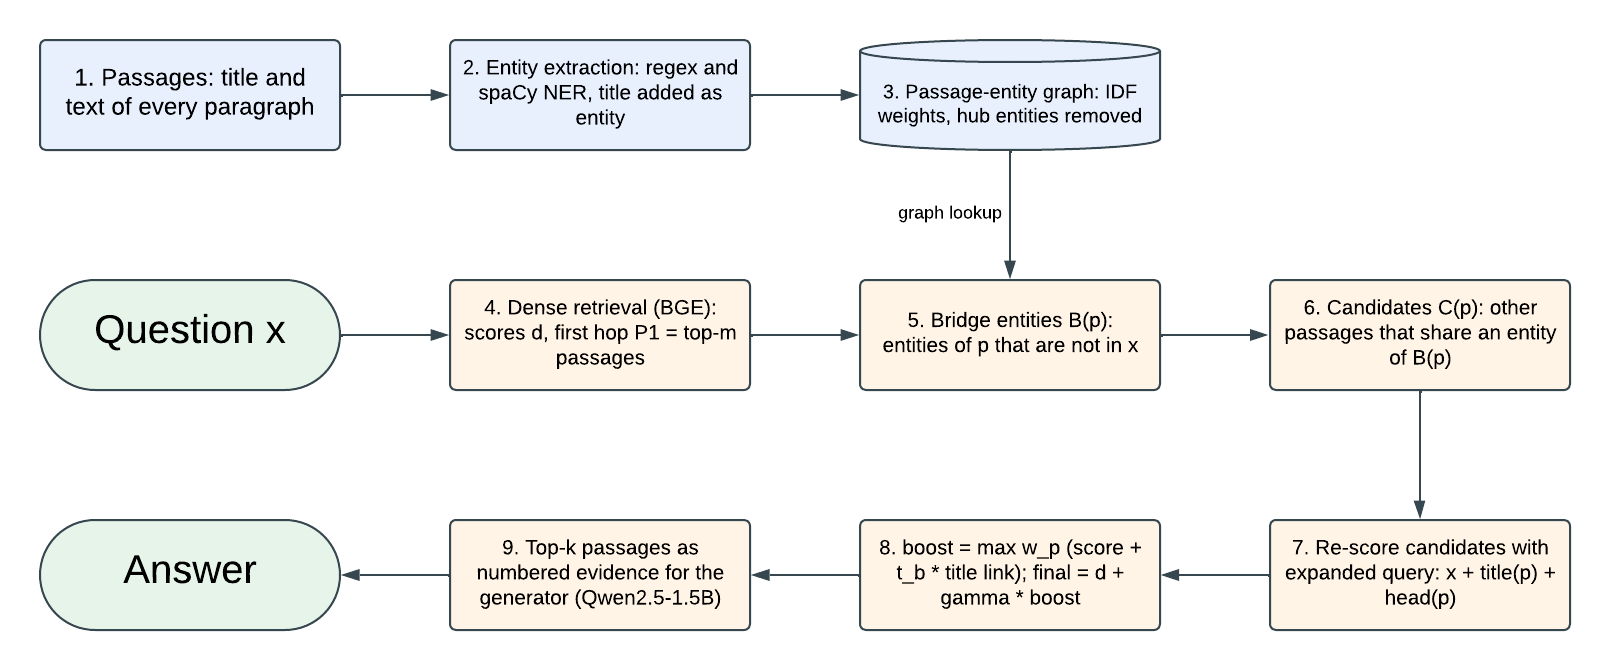
\includegraphics[width=\textwidth]{figs/pipeline_lucid.png}
\caption{Pipeline of the two-hop re-ranker (diagram drawn with Lucidchart). The dense retriever scores the question; the top-$m$ passages are the first hop. Their entities that are not in the question are bridge entities, which select candidate passages in the offline entity graph. Candidates are re-scored with a query expanded by the first-hop passage, and the boost is added to the dense score before the top-$k$ passages go to the generator.}
\label{fig:overview}
\end{figure}

\subsection{Offline stage: passage--entity graph}
Let $\mathcal{P}=\{p_1,\dots,p_n\}$ be the passages, each with a title and a text, and $\mathcal{E}=\{e_1,\dots,e_m\}$ the entities. An entity is found by a rule-based extractor (capitalised spans and four-digit years), by spaCy NER (\texttt{en\_core\_web\_sm}), or by the union of both; the passage title is always added as an entity of its passage. Entity strings are lower-cased and tokenised to form keys. Let $\mathrm{df}(e)$ be the number of passages containing $e$. The incidence matrix $A\in\mathbb{R}_{\ge0}^{n\times m}$ has $a_{pe}=w_e=\log(1+n/\mathrm{df}(e))$ if $e$ occurs in $p$. Entities with $\mathrm{df}(e)$ above one fifth of the passages are hubs, which link everything and carry no signal, so their edges are removed. The question entities $\mathcal{E}_x$ are the vocabulary entities that appear as token $n$-grams ($n\le4$) of $x$.

\subsection{Online stage: two-hop re-ranking}
For a question $x$ let $d(p)$ be the dense score and $\widetilde d$ its min--max normalisation over all passages. The first-hop set $P_1$ holds the $m$ passages with the highest $d$, each with weight $w_p=\exp\big((\widetilde d(p)-\max_{P_1}\widetilde d)/\tau\big)\in(0,1]$. For $p\in P_1$:
\begin{itemize}\setlength\itemsep{0pt}
\item \emph{Bridge entities} $B(p)$ are the entities of $p$ that are not in $\mathcal{E}_x$ (hubs were removed from the graph).
\item \emph{Candidates} $C(p)$ are the other passages that contain at least one entity of $B(p)$.
\item The \emph{expanded query} $x_p$ is $x$ followed by the title of $p$ and its first 40 words. Let $\widetilde d_p$ be the min--max normalised dense score of $x_p$ over all passages. The expanded query is therefore scored against the whole corpus (an exhaustive similarity computation, as for the question itself), but only the passages in $C(p)$ below can receive a boost.
\end{itemize}
The boost of a candidate is
\begin{equation}
\mathrm{boost}(c)=\max_{p\in P_1:\,c\in C(p)} w_p\big(\widetilde d_p(c)+t_b\,\mathbb{1}[\mathrm{title}(c)\in B(p)]\big),
\label{eq:boost}
\end{equation}
with $\mathrm{boost}(c)=0$ for passages in no $C(p)$. The final score is
\begin{equation}
\mathrm{score}(c)=\widetilde d(c)+\gamma\,\mathrm{boost}(c),
\label{eq:final}
\end{equation}
and the top-$k$ passages go to the generator as numbered passages. The title-link term rewards a candidate whose own title is one of the bridge entities, which is the typical pattern ``the first passage mentions the title of the second''.

\begin{algorithm}[t]
\caption{Graph-restricted two-hop re-ranking}\label{alg:two}
\KwIn{question $x$; graph $A$; dense scorer; $k,m,\gamma,t_b,\tau$}
\KwOut{top-$k$ passages}
$d\leftarrow$ dense scores of $x$; $\widetilde d\leftarrow$ min--max$(d)$; $P_1\leftarrow$ top-$m$ by $d$; $w_p\leftarrow\exp((\widetilde d(p)-\max\widetilde d)/\tau)$\;
\lIf{the gate fires}{\Return{top-$k$ by $d$}}
$\mathrm{boost}\leftarrow \mathbf 0$\;
\ForEach{$p\in P_1$}{
 $B\leftarrow$ entities of $p$ not in $\mathcal{E}_x$; $C\leftarrow$ passages sharing an entity with $B$, except $p$\;
 $\widetilde d_p\leftarrow$ min--max, over all passages, of the dense scores of $x\oplus\mathrm{title}(p)\oplus\mathrm{head}(p)$\;
 \ForEach{$c\in C$}{$\mathrm{boost}(c)\leftarrow\max\big(\mathrm{boost}(c),\,w_p(\widetilde d_p(c)+t_b\mathbb 1[\mathrm{title}(c)\in B])\big)$}}
\Return{top-$k$ of $\widetilde d+\gamma\,\mathrm{boost}$}
\end{algorithm}

\subsection{Question-type gate}\label{sec:gate}
The re-ranker helps bridge questions but hurts comparison questions, whose two entities are both named in the question (Section~\ref{sec:bytype}). The gate is a cheap test that returns the dense top-$k$ unchanged when it fires. The \emph{titles} gate fires when at least two of the dense top-$k$ passages have a title that is an entity of the question. The \emph{rule} gate fires when the question contains comparison cue words (for example ``both'', ``same'', ``older'', or two alternatives joined by ``or''). The gate is chosen among \{none, titles, rule\} by All@5 on the training sample only (Section~\ref{sec:hyper}); an \emph{oracle} gate that uses the gold question type is used only as an upper bound. When the gate fires, the ranking is identical to the dense ranking, and the extra encodings are skipped.

\subsection{Reduced variants: the expansion-only control and the title-link method}\label{sec:variants}
Equation~\eqref{eq:boost} has two terms that can be separated, and we add two reduced variants to find out which one does the work. They share the encoder, the first-hop set $P_1$, the weights $w_p$ and Equation~\eqref{eq:final}; only the boost differs.
\begin{itemize}\setlength\itemsep{0pt}
\item \emph{Title-link only}: $\mathrm{boost}(c)=\max_{p\in P_1} w_p\,t_b\,\mathbb{1}[\mathrm{title}(c)\in B(p)]$. The graph and the title match are kept, the expanded query is dropped. This variant needs no extra query encoding and no exhaustive scoring beyond the question itself.
\item \emph{Expansion only}: $\mathrm{boost}(c)=\max_{p\in P_1,\,c\ne p} w_p\,\widetilde d_p(c)$ for \emph{every} passage $c$. The expanded query is kept, scored against the whole corpus, and the graph and the title bonus are dropped, so the scoring budget equals that of the full method.
\end{itemize}
For each variant $\gamma$ is chosen on the training questions only (Section~\ref{sec:hyper}). Because the title-link boost is a constant for linked passages, the value of $\gamma t_b$ alone matters for it, and its training accuracy is flat for $\gamma\ge1$. We call the title-link variant \emph{TitleLink} and treat it as a principal method alongside the full two-hop method, not only as a control: it needs no extra query encoding, and Section~\ref{sec:controls} shows that it is stronger than the full method on HotpotQA and 2WikiMultiHopQA and weaker on MuSiQue.

\subsection{Earlier variant: PPR hybrid}\label{sec:ppr}
Our first design started a personalized PageRank walk on the bipartite graph. The restart distribution mixes question entities and the top dense passages, $\mathbf{s}=\lambda\,\mathbf{s}^{\mathrm{ent}}+(1-\lambda)\,\mathbf{s}^{\mathrm{den}}$ with $s^{\mathrm{den}}_p\propto\exp(d(p)/\tau)$ on the top-$s$ passages and $s^{\mathrm{ent}}_e\propto1/\log(1+\mathrm{df}(e))$ on $\mathcal{E}_x$. The PPR vector $\pi=\alpha\mathbf{s}+(1-\alpha)\pi P$, with $P$ the row-normalised transition matrix of the bipartite graph, is computed by power iteration, and the final score is $\beta\widetilde d+(1-\beta)\widetilde\pi$. In its generator prompt the retrieved passages are annotated with the entities that link them. We keep this variant as a baseline (``PPR hybrid'') and as the subject of the analysis in Section~\ref{sec:theory}.

\subsection{Design rationale}
Two observations motivate the design. First, in bridge questions the second supporting passage is usually named in the first one, often by its title, so an entity shared between the two is a cheap and fairly reliable link. Second, the dense score of the second passage against the question alone is low, but its score against the question \emph{plus the first passage} is high, because the first passage supplies the missing vocabulary. Using the graph only as a filter keeps the boost away from passages that are not linked to the first hop: such passages keep their dense score (Proposition~\ref{prop:boost}), although their rank can still fall when linked passages are lifted above them. The min--max normalisation puts the two dense scores on a common scale, and the weights $w_p$ make a lower-ranked first-hop passage contribute less. These two observations were our hypotheses, not findings. The controls of Section~\ref{sec:controls} test them separately and support the first (the title link) much more than the second (the expanded-query score).

\subsection{Generator prompt}
The generator receives the question and the numbered top-$k$ passages and is asked for the shortest answer supported by them. The two-hop re-ranker passes plain numbered passages; the PPR hybrid additionally annotates each passage with the entities that link it to the question.

\subsection{Complexity}
Graph construction needs one pass over the corpus for entity extraction and one sparse incidence matrix, so indexing costs $O(\mathrm{nnz}(A))$ memory and no model call beyond the optional spaCy tagger. At query time the re-ranker needs one dense scoring of the question and $m$ scorings of expanded queries, plus index look-ups (Proposition~\ref{prop:boost}). Each scoring is an exhaustive matrix--vector product over all $n$ passage embeddings, $O(n\,\delta)$ for embedding size $\delta$, followed by a min--max normalisation, so the query-time cost grows linearly with the corpus, as it does for exhaustive dense retrieval; the normalisation would have to be replaced to use an approximate nearest-neighbour index, which we did not test. With $m=\tTwoM$ the number of query encodings is $\tTwoM+1$ per question; the measured wall-clock cost is given in Section~\ref{sec:cost}.

\section{Theoretical Analysis}\label{sec:theory}
\begin{proposition}[Guaranteed boost and cost of the re-ranker]\label{prop:boost}
Let $c\ne p$ be a passage and $p\in P_1$. (a) If $c$ lies in no $C(p')$, then $\mathrm{score}(c)=\widetilde d(c)$: such passages keep their dense score and their order relative to one another, but their rank in the final list can fall when linked passages are boosted above them. (b) If $\mathrm{title}(c)\in B(p)$ and the title entity of $c$ is not a hub, then $c\in C(p)$ and $\mathrm{score}(c)\ \ge\ \widetilde d(c)+\gamma\,w_p\,t_b$. (c) The method adds $|P_1|=m$ dense query encodings, each followed by one similarity scoring against all $n$ passages (needed for the min--max normalisation), and $O\big(\sum_{p\in P_1}\sum_{e\in B(p)}\mathrm{df}(e)\big)$ index lookups per question; no LLM call is made.
\end{proposition}
\begin{pf}
(a) holds because $\mathrm{boost}(c)=0$ by definition. (b) The title of $c$ is an entity of $c$, so $c$ contains an entity of $B(p)$ and lies in $C(p)$; the indicator in Eq.~\eqref{eq:boost} is one and $\widetilde d_p(c)\ge0$, so $\mathrm{boost}(c)\ge w_pt_b$ and Eq.~\eqref{eq:final} gives the claim. (c) is read off Algorithm~\ref{alg:two}.
\end{pf}
When the gate of Section~\ref{sec:gate} fires, the output is the dense top-$k$, so the guarantees above apply only to questions the gate lets through. The proposition says what the re-ranker can and cannot do. A passage that names a first-hop bridge entity in its title is raised by a fixed margin that does not depend on lexical overlap with the question, while the \emph{scores} of unlinked passages are unchanged, so the graph can lift only linked evidence; an unlinked passage can still lose rank when linked passages are lifted above it. It does not say that the boosted passage becomes relevant; whether the boost helps is an empirical question (Section~\ref{sec:results}). The bounds below concern the earlier PPR variant.

\subsection{PPR variant}
We analyse the retrieval step. Throughout, the graph is the one in Section~\ref{sec:method}, nodes with no incident edge (for example entities removed as hubs) are deleted, and $P$ is therefore row-stochastic. For a restart distribution $\mathbf{s}$ and $\alpha\in(0,1)$ the PPR vector is
\begin{equation}
\pi=\alpha\sum_{t=0}^{\infty}(1-\alpha)^t\,\mathbf{s}P^t .
\label{eq:pprseries}
\end{equation}

\begin{proposition}[Path mass]\label{prop:path}
For any walk $v_0,v_1,\dots,v_t$ in the graph,
\[\pi(v_t)\ \ge\ \alpha(1-\alpha)^t\,s(v_0)\prod_{i=1}^{t}P(v_{i-1},v_i).\]
\end{proposition}
\begin{pf}
All terms of~\eqref{eq:pprseries} are nonnegative, so $\pi(v_t)$ is at least its $t$-th term, $\alpha(1-\alpha)^t(\mathbf{s}P^t)(v_t)$. The entry $(\mathbf{s}P^t)(v_t)$ is the sum over all length-$t$ walks ending in $v_t$ of the start mass times the transition probabilities, and a single walk contributes the product in the statement.
\end{pf}

\begin{corollary}[Two-hop bridge]\label{cor:bridge}
Let $q$ be a seed entity and $p_1,p_2$ passages that both contain an entity $e$, with $q\in p_1$. Then
\[
\pi(p_2)\ \ge\ \alpha(1-\alpha)^3\, s(q)\ \frac{1}{\mathrm{df}(q)}\ \frac{w_e}{\sum_{e'\in p_1}w_{e'}}\ \frac{1}{\mathrm{df}(e)} .
\]
\end{corollary}
\begin{pf}
Apply Proposition~\ref{prop:path} to the walk $q\to p_1\to e\to p_2$ with the transition probabilities $P(q,p_1)=1/\mathrm{df}(q)$, $P(p_1,e)=w_e/\sum_{e'\in p_1}w_{e'}$ and $P(e,p_2)=1/\mathrm{df}(e)$, which follow from the weights.
\end{pf}

\begin{remark}
The bound is positive whenever the passages are connected through a shared entity, whatever the lexical overlap between the question and $p_2$, which is the case where scoring $p_2$ against the question alone gives no guarantee. It also shows how the weights act. A rare bridge entity (small $\mathrm{df}(e)$, large $w_e$) transmits more mass, while a hub entity transmits little, which motivates the IDF weights and the hub threshold. The bound is a lower bound from one path; it does not say that $p_2$ is ranked above all distractors, and the fusion with the dense score and the experiments address that part.
\end{remark}

\begin{proposition}[Convergence and cost]\label{prop:conv}
Let $\pi_0=\mathbf{s}$ and $\pi_{t+1}=\alpha\mathbf{s}+(1-\alpha)\pi_tP$. Then $\|\pi_T-\pi\|_1\le 2(1-\alpha)^T$, so $T\ge\ln(2/\varepsilon)/\alpha$ iterations give $\ell_1$ error at most $\varepsilon$. Each iteration costs $O(\mathrm{nnz}(A))$.
\end{proposition}
\begin{pf}
The fixed-point equation gives $\pi_{t+1}-\pi=(1-\alpha)(\pi_t-\pi)P$. A row-stochastic $P$ does not increase the $\ell_1$ norm, so $\|\pi_T-\pi\|_1\le(1-\alpha)^T\|\mathbf{s}-\pi\|_1\le 2(1-\alpha)^T$, because both vectors are probability distributions. The bound on $T$ follows from $(1-\alpha)^T\le e^{-\alpha T}$. One multiplication by $P$ touches each nonzero of $A$ twice.
\end{pf}

\section{Experimental Setup}\label{sec:setup}
\subsection{Data and corpora}
We use the HotpotQA distractor development set \citep{yang2018hotpotqa}. A sample of 1\,000 questions (fixed seed) has its paragraphs pooled into one de-duplicated corpus (\nPHotpotQA{} paragraphs for sample A), so retrieval must find evidence among the paragraphs of other questions as well. Sample A (seed 0) was used for development comparisons of the PPR variant; sample B (seed 1, a second random draw of 1\,000 questions; \nOverlapAB{} questions occur in both samples) was first run once for the frozen ungated configuration, after all settings were fixed, and later reused for the gate and the cross-encoder (Section~\ref{sec:evalprot}). HotpotQA questions are of two types, bridge and comparison \citep{yang2018hotpotqa}. For transfer we use 1\,000 random questions each from the validation split of 2WikiMultiHopQA \citep{ho2020twowiki} (compositional, inference, comparison and bridge-comparison questions; 6\,223 pooled paragraphs) and from the answerable dev split of MuSiQue \citep{trivedi2022musique} (2- to 4-hop questions; 11\,525 pooled paragraphs), built in the same way. All pooled corpora are smaller than open-domain retrieval over Wikipedia (Section~\ref{sec:discussion}).

\subsection{Compared systems}
\emph{No retrieval}; \emph{BM25} \citep{robertson2009bm25}; \emph{Dense}, the BGE-small-en-v1.5 bi-encoder \citep{xiao2023bge}; \emph{Graph-PPR} (entity seeds only); the \emph{PPR hybrid} (Section~\ref{sec:ppr}); the proposed \emph{two-hop re-ranking} with and without the question-type gate (Section~\ref{sec:gate}); and \emph{gold passages} as an upper bound. As a re-ranking baseline we use a \emph{cross-encoder}, \texttt{bge-reranker-base} \citep{xiao2023bge}, which re-scores the top-20 passages of a first-stage retriever \citep{nogueira2019rerank}; we apply it to the dense top-20 (``CE (dense)'') and to the top-20 of the two-hop re-ranker (``CE (two-hop)''). All retrievers that use a dense score share the same encoder. Ablations of the re-ranker remove the title-link bonus ($t_b=0$), use only the top-1 first-hop passage ($m=1$), or use regex entities only. An \emph{oracle gate}, which uses the gold question type, is reported as an upper bound for the gate only. Official GraphRAG, LightRAG and HippoRAG are not run and are not compared; running them requires an LLM at indexing time, which was outside our compute budget.

\subsection{Implementation details}
The dense encoder is BGE-small-en-v1.5 with its query instruction prefix, loaded through the Transformers library \citep{wolf2020transformers}. Entities come from the rule-based extractor and from spaCy \texttt{en\_core\_web\_sm} (version 3.8). The generator is Qwen2.5-1.5B-Instruct \citep{qwen2024qwen25} in half precision with greedy decoding and at most 32 new tokens. The main experiments (the two HotpotQA samples, the cross-encoder runs, 2WikiMultiHopQA, MuSiQue and the answer generation) ran on a single Apple M4 laptop (GPU through the Metal backend, no external API). The TitleLink retrieval, the answers of all systems on both samples, the re-implemented LinearRAG- and SPRIG-style baselines and the common-pool comparison of Section~\ref{sec:gpu} ran on a single NVIDIA H200 GPU server with the same code and models (retrieval results are identical to the laptop's). The controls, candidate-coverage, audit, corpus-scale and repeated-timing experiments of Sections~\ref{sec:controls} and~\ref{sec:cost} were rerun on a two-core cloud CPU container with the same code, encoder and models; their numbers are reported separately and not mixed with the laptop timings, and the CPU results for dense, two-hop and gated retrieval reproduce the laptop All@5 to within rounding (Table~\ref{tab:controls}). The fixed settings are $k=5$, $\tau=0.1$, 40 expansion words and a hub threshold of 20\% of the passages. Every table and macro in this paper is produced from the stored per-question result files by the released scripts.

\subsection{Hyper-parameter and gate selection}\label{sec:hyper}
Both methods were tuned on HotpotQA \emph{training} questions (\tTuneN{} questions with their own pooled corpus), never on the evaluation sets. The PPR hybrid used $\alpha\in\{0.15,0.3\}$, $\lambda\in\{0.25,0.5,0.75\}$, $\beta\in\{0.3,0.5,0.7\}$ and selected $\alpha=\tAlpha$, $\lambda=\tLam$, $\beta=\tBeta$. The re-ranker used $m\in\{2,3\}$, $\gamma\in\{0.1,0.2,0.3,0.5,1,2\}$, $t_b\in\{0,0.5\}$ and the entity extractor in \{regex, spaCy, both\}, and selected $m=\tTwoM$, $\gamma=\tTwoGamma$, $t_b=\tTwoTb$ and extractor \texttt{\tTwoNer}. The first sweep covered $\gamma\in\{0.5,1,2\}$ and placed the optimum at the lower edge, so a second sweep of $\{0.1,0.2,0.3\}$ was added, again on the training sample only. On the training sample the selected configuration reaches All@5 of \tTwoAll\% against \tTwoDense\% for dense retrieval. With these settings frozen, the gate was selected on the same training sample from \{none, titles, rule\}: All@5 was \GateNoneTrain\%, \GateTitlesTrain\% and \GateRuleTrain\% respectively, so the \texttt{\GateChosen} gate was chosen (it fires for \GateTitlesShare\% of training questions). The oracle gate (\GateOracleTrain\%) was never a candidate. The two controls of Section~\ref{sec:variants} were tuned in the same way on the same training sample (\ClTrainN{} questions, \ClTrainP{} passages): $\gamma\in\{0.1,0.2,0.3,0.5,1,1.5,2,3,5\}$ for each variant with $m=\tTwoM$ and $t_b=\tTwoTb$ fixed. Training All@5 of the expansion-only control peaks at $\gamma=\CtlGammaExp$ (\CtlTrainExpAll\%), against \ClDenseTrain\% for dense retrieval; the title-link-only control reaches \CtlTrainTitAll\% from $\gamma=\CtlGammaTit$ upward and is flat beyond (the constant boost already moves every linked passage above the dense scores), so the smallest value of that plateau was chosen; and the full method peaks at \CtlTrainTwoAll\% at $\gamma=\tTwoGamma$. A first run used the narrower grid $\gamma\le1$ and put the optimum of the title-link control at the upper edge; the grid was then widened (the first-grid results are kept in the released files). The selection itself uses training questions only. No setting was tuned on 2WikiMultiHopQA or MuSiQue.

\subsection{Evaluation protocol}\label{sec:evalprot}
Sample B had been run once with the frozen ungated configuration before the gate and the cross-encoder were added. The extended runs reuse samples A and B and add the new systems to them; because the gate was selected on training data and the cross-encoder was not tuned, this does not use the evaluation labels for selection, but sample B should no longer be read as a sample that was seen exactly once by every system. 2WikiMultiHopQA and MuSiQue were each run once, retrieval only. The generator was run on sample A for no retrieval, BM25, dense retrieval, the PPR hybrid, the re-ranker, the gated re-ranker, the cross-encoder on dense and gold passages.

\subsection{Evaluation metrics}
\paragraph{Retrieval.} Recall of supporting passages in the top-5 (R@5) and the share of questions for which all supporting passages are retrieved (All@5). On MuSiQue up to four passages are supporting, so All@5 is very strict for 3- and 4-hop questions.
\paragraph{Answers.} Exact match (EM) and token-level F1 after the usual normalisation \citep{rajpurkar2016squad}.
\paragraph{Groundedness.} The rate of answers for which less than 0.8 of the content tokens occur in the retrieved evidence, reported as ``Unsup.'' (lower is better). This is a lexical proxy, not an entailment-based or claim-level faithfulness score \citep{honovich2022true,min2023factscore}.

\subsection{Statistical testing}
Differences between systems on the same questions are tested with a paired bootstrap \citep{efron1979bootstrap,berg2012bootstrap,koehn2004signif} with 10\,000 resamples over questions; we report the mean difference, the 95\% percentile interval and a two-sided $p$ value. No correction is made for the number of comparisons.

\section{Results}\label{sec:results}
\IfFileExists{tables/retr2.tex}{\begin{table}[t]
\centering
\small
\caption{Retrieval on two random samples (159 questions in common) of 1\,000 HotpotQA questions (\%). Sample~A was also used to evaluate the earlier PPR variant; sample~B was first run once with the frozen ungated configuration and later reused (Section~\ref{sec:evalprot}). Best non-oracle value in bold.}
\label{tab:retr2}
\begin{tabular}{lrrrr}
\toprule
System & \multicolumn{2}{c}{SampleA} & \multicolumn{2}{c}{SampleB} \\
& R@5 & All@5 & R@5 & All@5 \\
\midrule
BM25 & 73.8 & 51.3 & 71.6 & 48.1 \\
Dense & 84.3 & 70.2 & 84.1 & 69.8 \\
PPR hybrid (v1) & 84.3 & 70.1 & 84.0 & 69.8 \\
Two-hop graph re-ranking (ours) & 88.1 & 78.6 & \textbf{88.8} & \textbf{80.3} \\
w/o title-link bonus & 85.5 & 73.5 & 85.4 & 73.4 \\
first hop from top-1 only & 84.7 & 73.5 & 85.9 & 76.1 \\
regex entities only & \textbf{88.2} & \textbf{78.8} & 88.6 & 79.8 \\
Gold passages (upper bound) & 100.0 & 100.0 & 100.0 & 100.0 \\
\bottomrule
\end{tabular}
\end{table}}{}

\subsection{Retrieval quality (RQ1)}
Table~\ref{tab:retr2} gives retrieval on the two HotpotQA samples. The two-hop re-ranker retrieves all supporting passages for \RSampleAHybridTwoAllSupp\% (sample A) and \RSampleBHybridTwoAllSupp\% (sample B) of the questions, against \RSampleADenseAllSupp\% and \RSampleBDenseAllSupp\% for dense retrieval and \RSampleABmTwoAllSupp\% and \RSampleBBmTwoAllSupp\% for BM25. Recall in the top-5 rises from \RSampleADenseRecall\% to \RSampleAHybridTwoRecall\% and from \RSampleBDenseRecall\% to \RSampleBHybridTwoRecall\%. The gain is similar on the second sample, which supports the claim that it is not an artefact of development on sample A. The paired bootstrap in Table~\ref{tab:signif} excludes zero for every retrieval comparison. In contrast, the PPR hybrid is indistinguishable from dense retrieval (All@5 \RSampleAHybridAllSupp\% against \RSampleADenseAllSupp\% on sample A and \RSampleBHybridAllSupp\% against \RSampleBDenseAllSupp\% on sample B), and Graph-PPR with entity seeds alone reaches only \RHotpotQAGraphAllSupp\% (Table~\ref{tab:main}). The graph walk therefore did not help on top of BGE, whereas the same graph used to restrict a second dense scoring pass did.

\IfFileExists{tables/signif.tex}{\begin{table}[t]
\centering
\small
\caption{Paired bootstrap (10\,000 resamples) of Two-hop graph re-ranking (ours) versus Dense: mean difference in percentage points, 95\% CI and two-sided $p$.}
\label{tab:signif}
\begin{tabular}{llrrr}
\toprule
Dataset & Metric & $\Delta$ & 95\% CI & $p$ \\
\midrule
HotpotQA (sample A) & R@5 & +3.9 & [+2.5, +5.3] & <0.001 \\
HotpotQA (sample A) & All@5 & +8.4 & [+5.7, +11.1] & <0.001 \\
HotpotQA (sample A) & EM & +5.0 & [+2.8, +7.4] & <0.001 \\
HotpotQA (sample A) & F1 & +5.5 & [+3.2, +7.8] & <0.001 \\
HotpotQA (sample A) & Unsup.$\downarrow$ & -1.2 & [-2.7, +0.3] & 0.117 \\
HotpotQA (sample B) & R@5 & +4.7 & [+3.3, +6.1] & <0.001 \\
HotpotQA (sample B) & All@5 & +10.5 & [+7.8, +13.2] & <0.001 \\
\bottomrule
\end{tabular}
\end{table}}{}

\subsection{Ablation (RQ2)}
Removing the title-link bonus lowers All@5 to \RSampleAAblTwoNoTitleAllSupp\% (sample A) and \RSampleBAblTwoNoTitleAllSupp\% (sample B), and using only the top-1 first-hop passage gives \RSampleAAblTwoOneSeedAllSupp\% and \RSampleBAblTwoOneSeedAllSupp\%, so both the title link and several first-hop passages contribute. Restricting entities to the regex extractor gives \RSampleAAblTwoRegexNerAllSupp\% and \RSampleBAblTwoRegexNerAllSupp\%, which is equal to the selected union with spaCy within sampling noise; spaCy therefore does not add measurable value here, and the cheaper extractor suffices. The ablations of the PPR variant (Table~\ref{tab:ablation}) show that dropping the dense seeds is damaging (All@5 \RHotpotQAAblNoDenseSeedAllSupp\%), dropping the dense-score fusion costs about two points (\RHotpotQAAblNoFusionAllSupp\%), and removing the entity seeds (\RHotpotQAAblNoEntitySeedAllSupp\%), the IDF weights (\RHotpotQAAblNoIdfAllSupp\%) or changing the restart probability (\RHotpotQAAblAlphaZeroAllSupp\%) stays within one point of the full PPR hybrid (\RHotpotQAHybridAllSupp\%), which itself equals dense retrieval.

\IfFileExists{tables/ablation.tex}{\begin{table}[t]
\centering
\small
\caption{Ablation of the earlier PPR hybrid (\%); the PPR variant was not run with the generator except in its full form.}
\label{tab:ablation}
\begin{tabular}{llrrrrr}
\toprule
Dataset & System & R@5 & All@5 & EM & F1 & Unsup.$\downarrow$ \\
\midrule
\multirow{6}{*}{HotpotQA} & PPR hybrid (v1) & 84.3 & 70.1 & \textbf{36.6} & \textbf{46.8} & \textbf{12.2} \\
 & w/o entity seeds & \textbf{84.7} & \textbf{71.0} & -- & -- & -- \\
 & w/o dense seeds & 69.0 & 47.2 & -- & -- & -- \\
 & w/o dense-score fusion & 83.2 & 68.1 & -- & -- & -- \\
 & w/o IDF edge weights & 84.5 & 70.5 & -- & -- & -- \\
 & restart $\alpha=0.5$ & 84.3 & 70.3 & -- & -- & -- \\
\bottomrule
\end{tabular}
\end{table}}{}

\subsection{Error analysis and the question-type gate (RQ3)}\label{sec:bytype}
\begin{table*}[t]
\centering
\scriptsize
\caption{All@5 (\%) by question type. CE: cross-encoder. The gate restores comparison questions to about the dense level. Two-hop re-ranking gains on bridge, compositional, inference and 2-hop questions, but not on 3-hop or 4-hop MuSiQue questions (it loses on 3-hop).}
\label{tab:bytype2}
\begin{tabular}{lrrrrrrrrrrr}
\toprule
 & \multicolumn{2}{c}{HotpotQA A} & \multicolumn{2}{c}{HotpotQA B} & \multicolumn{4}{c}{2WikiMultiHopQA} & \multicolumn{3}{c}{MuSiQue} \\
System & bridge & compar. & bridge & compar. & compos. & infer. & compar. & br.-cmp. & 2-hop & 3-hop & 4-hop \\
\midrule
$n$ & 792 & 208 & 784 & 216 & 413 & 115 & 232 & 240 & 518 & 304 & 178 \\
\midrule
Dense & 62.5 & 99.5 & 61.7 & 99.1 & 26.6 & 39.1 & 97.8 & 0.0 & 26.1 & 5.9 & 0.0 \\
CE (dense top-20) & 76.3 & 100.0 & 75.9 & 99.5 & 26.6 & 40.0 & 99.6 & 0.0 & 29.7 & 8.2 & 0.6 \\
Two-hop & 75.8 & 89.4 & 77.7 & 89.8 & 73.6 & 66.1 & 89.7 & 2.5 & 39.8 & 3.3 & 0.0 \\
Two-hop + gate & 74.9 & 97.6 & 77.3 & 97.2 & 73.4 & 66.1 & 97.0 & 0.4 & 40.0 & 3.6 & 0.0 \\
CE (two-hop top-20) & 82.1 & 97.6 & 83.4 & 99.1 & 45.3 & 50.4 & 98.3 & 0.4 & 36.9 & 12.5 & 0.0 \\
CE (gated two-hop) & 81.9 & 100.0 & 83.0 & 99.5 & 44.8 & 50.4 & 99.6 & 0.0 & 36.5 & 12.5 & 0.6 \\
Two-hop + oracle gate & 75.8 & 99.5 & 77.7 & 99.1 & 73.6 & 66.1 & 97.8 & 0.0 & 39.8 & 3.3 & 0.0 \\
\bottomrule
\end{tabular}
\end{table*}
Table~\ref{tab:bytype2} splits All@5 by question type. On HotpotQA the whole gain of the ungated re-ranker comes from bridge questions, where All@5 rises from \TypHADensebridge\% to \TypHATwobridge\% on sample A ($n=\TypNHAbridge$) and from \TypHBDensebridge\% to \TypHBTwobridge\% on sample B ($n=\TypNHBbridge$). On comparison questions the ungated re-ranker is \emph{worse}: All@5 falls from \TypHADensecomparison\% to \TypHATwocomparison\% on sample A ($n=\TypNHAcomparison$) and from \TypHBDensecomparison\% to \TypHBTwocomparison\% on sample B ($n=\TypNHBcomparison$). The same drop appears on the comparison questions of 2WikiMultiHopQA (\TypTWDensecomparison\% to \TypTWTwocomparison\%). A comparison question names both entities, so the dense retriever already finds both passages, and our hypothesis is that the boost for linked passages then displaces one of them from the top-5. We did not test this explanation directly.

The question-type gate of Section~\ref{sec:gate} removes most of the loss. With the gate, comparison questions are at \TypHAGatecomparison\% (sample A), \TypHBGatecomparison\% (sample B) and \TypTWGatecomparison\% (2WikiMultiHopQA), close to dense retrieval and to the oracle gate (\TypHAOraccomparison\% on sample A), and the gate fires for \ExtHAGateGated\% of the questions on sample A. Overall All@5 rises from \ExtHATwoAll\% to \ExtHAGateAll\% on sample A and from \ExtHBTwoAll\% to \ExtHBGateAll\% on sample B. The paired differences are \ExtHAGateVTwoAllD{} points (95\% interval \ExtHAGateVTwoAllLo{} to \ExtHAGateVTwoAllHi{}) on sample A, which includes zero, and \ExtHBGateVTwoAllD{} points (\ExtHBGateVTwoAllLo{} to \ExtHBGateVTwoAllHi{}) on sample B, which does not (Table~\ref{tab:extsig}). The gate is therefore a small but consistent repair, not a large gain. It is imperfect: the title-based gate loses about one point on bridge questions on sample A (\TypHATwobridge\% to \TypHAGatebridge\%), and the oracle gate would add a further point or so (\ExtHAOracAll\% against \ExtHAGateAll\% on sample A).

The win--loss counts of the ungated re-ranker agree with this picture. On sample A, both systems retrieve all supporting passages for \WABoth{} questions, the dense retriever alone for \WADenseOnly{}, the re-ranker alone for \WAHtwoOnly{}, and neither for \WANeither{}; on sample B the counts are \WBBoth{}, \WBDenseOnly{}, \WBHtwoOnly{} and \WBNeither{}. The re-ranker thus fixes roughly two and a half to three times as many questions as it breaks.

\subsection{Comparison with a cross-encoder (RQ4)}
\begin{table*}[t]
\centering
\footnotesize
\caption{Retrieval with two-hop re-ranking, a question-type gate and a cross-encoder on four evaluation sets (\%; 1\,000 questions each). Settings were frozen from HotpotQA training data; 2WikiMultiHopQA and MuSiQue are zero-shot transfer. Sec.: retrieval time for 1\,000 questions on the H200 server. Best non-oracle value per column in bold.}
\label{tab:ext}
\begin{tabular}{lrrrrrrrrrrrr}
\toprule
System & \multicolumn{3}{c}{HotpotQA A} & \multicolumn{3}{c}{HotpotQA B} & \multicolumn{3}{c}{2Wiki} & \multicolumn{3}{c}{MuSiQue} \\
& R@5 & All@5 & Sec. & R@5 & All@5 & Sec. & R@5 & All@5 & Sec. & R@5 & All@5 & Sec. \\
\midrule
BM25 & 73.8 & 51.3 & 1 & 71.6 & 48.1 & 1 & 65.6 & 31.7 & 1 & 43.6 & 10.0 & 2 \\
Dense & 84.3 & 70.2 & 4 & 84.1 & 69.8 & 78 & 69.5 & 38.2 & 4 & 49.8 & 15.3 & 4 \\
\midrule
CE (dense top-20) & 90.2 & 81.2 & 46 & 90.0 & 81.0 & 94 & 70.2 & 38.7 & 58 & 53.7 & 18.0 & 46 \\
Two-hop & 88.1 & 78.6 & 22 & 88.8 & 80.3 & 21 & \textbf{80.8} & 59.4 & 17 & 48.3 & 21.6 & 22 \\
Two-hop + gate & 88.6 & 79.6 & 18 & 89.5 & 81.6 & 69 & 80.6 & \textbf{60.5} & 12 & 49.2 & 21.8 & 19 \\
\midrule
CE (two-hop top-20) & 92.2 & 85.3 & 72 & \textbf{92.8} & \textbf{86.8} & 71 & 75.0 & 47.4 & 80 & 54.4 & \textbf{22.9} & 72 \\
CE (gated two-hop) & \textbf{92.3} & \textbf{85.7} & 66 & 92.7 & 86.6 & 66 & 74.7 & 47.4 & 72 & \textbf{54.9} & 22.8 & 68 \\
Two-hop + oracle gate & 89.2 & 80.7 & 17 & 89.8 & 82.3 & 17 & 80.4 & 60.7 & 11 & 48.3 & 21.6 & 21 \\
\bottomrule
\end{tabular}
\end{table*}
Table~\ref{tab:ext} adds a cross-encoder re-ranker. On HotpotQA the cross-encoder over the dense top-20 improves All@5 from \ExtHADenseAll\% to \ExtHACEAll\% on sample A and from \ExtHBDenseAll\% to \ExtHBCEAll\% on sample B. The two-hop re-ranker with the gate reaches \ExtHAGateAll\% and \ExtHBGateAll\%. In All@5 the difference between the two is not significant on either sample (\ExtHAGateVCEAllD{} points, interval \ExtHAGateVCEAllLo{} to \ExtHAGateVCEAllHi{} on sample A; \ExtHBGateVCEAllD{} points, \ExtHBGateVCEAllLo{} to \ExtHBGateVCEAllHi{} on sample B), although the cross-encoder has slightly higher recall on sample A (\ExtHAGateVCERecD{} points for the gated method, interval \ExtHAGateVCERecLo{} to \ExtHAGateVCERecHi{}). The two methods cost very different amounts: the cross-encoder takes \ExtHACESec\,s per 1\,000 questions against \ExtHAGateSec\,s for the gated re-ranker in the single laptop run, and the repeated CPU measurements of Section~\ref{sec:cost} confirm the direction, because it scores 20 passage--question pairs per question.

The two methods are complementary on HotpotQA. Applying the cross-encoder to the top-20 of the gated re-ranker raises All@5 to \ExtHACEGateAll\% on sample A and \ExtHBCEGateAll\% on sample B, which is \ExtHACEGateVCEAllD{} and \ExtHBCEGateVCEAllD{} points over the cross-encoder alone (intervals above zero in both cases, Table~\ref{tab:extsig}). The picture differs on 2WikiMultiHopQA. There the cross-encoder gives no gain over dense retrieval (\ExtTWDenseAll\% to \ExtTWCEAll\%), whereas the two-hop re-ranker raises All@5 to \ExtTWTwoAll\%. Placing the cross-encoder \emph{after} the two-hop step still beats the cross-encoder alone (\ExtTWCETwoAll\%) but falls well below the two-hop step alone, mainly on compositional questions (\TypTWTwocompositional\% to \TypTWCETwocompositional\%, Table~\ref{tab:bytype2}). A plausible reason is that a cross-encoder trained to match a question with a passage ranks the bridge passage, which shares little with the question, below distractors, but we did not test this. The two re-rankers should therefore not be stacked without checking the dataset.

\IfFileExists{tables/ext_signif.tex}{\begin{table*}[t]
\centering
\scriptsize
\setlength{\tabcolsep}{3pt}
\caption{Paired bootstrap (10\,000 resamples) for All@5: mean difference in points with 95\% interval. An interval that excludes zero corresponds to $p<0.05$.}
\label{tab:extsig}
\begin{tabular}{lrrrr}
\toprule
Comparison & HotpotQA A & HotpotQA B & 2Wiki & MuSiQue \\
\midrule
Two-hop vs Dense & +8.4 [+5.7, +11.1] & +10.5 [+7.8, +13.2] & +21.2 [+18.3, +24.1] & +6.3 [+3.9, +8.7] \\
CE (dense top-20) vs Dense & +11.0 [+8.8, +13.3] & +11.2 [+8.8, +13.6] & +0.5 [$-$1.2, +2.2] & +2.7 [+0.8, +4.7] \\
Two-hop vs CE (dense top-20) & $-$2.6 [$-$5.3, +0.2] & $-$0.7 [$-$3.3, +1.9] & +20.7 [+17.7, +23.6] & +3.6 [+0.9, +6.2] \\
CE (two-hop top-20) vs CE (dense top-20) & +4.1 [+2.3, +5.9] & +5.8 [+4.0, +7.6] & +8.7 [+6.9, +10.6] & +4.9 [+3.0, +6.8] \\
Two-hop + gate vs Two-hop & +1.0 [$-$0.1, +2.1] & +1.3 [+0.3, +2.3] & +1.1 [+0.2, +2.0] & +0.2 [$-$0.5, +0.9] \\
Two-hop + gate vs Dense & +9.4 [+7.0, +11.9] & +11.8 [+9.3, +14.2] & +22.3 [+19.6, +25.0] & +6.5 [+4.2, +8.8] \\
Two-hop + gate vs CE (dense top-20) & $-$1.6 [$-$4.2, +1.0] & +0.6 [$-$1.9, +3.1] & +21.8 [+19.0, +24.6] & +3.8 [+1.2, +6.3] \\
CE (gated two-hop) vs CE (dense top-20) & +4.5 [+2.8, +6.2] & +5.6 [+3.9, +7.4] & +8.7 [+6.9, +10.5] & +4.8 [+3.0, +6.6] \\
CE (two-hop top-20) vs Two-hop & +6.7 [+4.2, +9.1] & +6.5 [+4.0, +8.9] & $-$12.0 [$-$14.7, $-$9.3] & +1.3 [$-$1.2, +3.8] \\
\bottomrule
\end{tabular}
\end{table*}}{}

\subsection{Transfer to 2WikiMultiHopQA and MuSiQue (RQ5)}
With the settings frozen on HotpotQA training data, the two-hop re-ranker transfers to both datasets (Table~\ref{tab:ext}). On 2WikiMultiHopQA All@5 rises from \ExtTWDenseAll\% to \ExtTWTwoAll\% (\ExtTWTwoVDenseAllD{} points, interval \ExtTWTwoVDenseAllLo{} to \ExtTWTwoVDenseAllHi{}), and to \ExtTWGateAll\% with the gate; recall rises from \ExtTWDenseRec\% to \ExtTWTwoRec\%. The gain is largest for compositional questions (\TypTWDensecompositional\% to \TypTWTwocompositional\%) and also clear for inference questions (\TypTWDenseinference\% to \TypTWTwoinference\%). All systems score close to zero on the bridge-comparison questions ($n=\TypNTWbridgecomparison$); Section~\ref{sec:controls} shows that this is not an evaluation error: every such question has a supporting set of \AudSizeBridgecomparison{} passages, which fits in five, but dense retrieval finds all four for \AudDenseBridgecomparisonAll\% of them (\AudDenseBridgecomparisonAllTwenty\% at 20).

On MuSiQue the result is mixed. All@5 rises from \ExtMQDenseAll\% to \ExtMQTwoAll\% (\ExtMQTwoVDenseAllD{} points, interval \ExtMQTwoVDenseAllLo{} to \ExtMQTwoVDenseAllHi{}), but recall in the top-5 does not (\ExtMQDenseRec\% to \ExtMQTwoRec\%, difference \ExtMQTwoVDenseRecD{} points, interval \ExtMQTwoVDenseRecLo{} to \ExtMQTwoVDenseRecHi{}), and the cross-encoder has higher recall than the two-hop method (\ExtMQCERec\%). The gain comes from 2-hop questions (\TypMQDenseTwohop\% to \TypMQTwoTwohop\%). For 3-hop questions the re-ranker is worse than dense retrieval (\TypMQDenseThreehop\% to \TypMQTwoThreehop\%) and for 4-hop questions all systems are near zero. The method, which follows one bridge from the first hop, does not recover chains of three or more supporting passages in this setup. The gate has no measurable effect on MuSiQue (\ExtMQGateAll\%), as expected from a dataset without comparison questions.

\subsection{Controls, candidate coverage, audit and scale}\label{sec:controls}
\paragraph{What does the graph add? (controls).}
Tables~\ref{tab:controls} and~\ref{tab:controlsgate} separate query expansion from the graph and title link (Section~\ref{sec:variants}); the paired differences are in Table~\ref{tab:ctlsig}. Scoring the same expanded queries against the whole corpus, without the graph, raises HotpotQA sample A from \CtlHADenseAll\% to only \CtlHAExpFAll\%, far below the full method (\CtlHATwoFAll\%); the graph restriction is therefore needed for the expansion to help. The reverse control is more important: keeping only the graph and the title link, with no expanded query, reaches \CtlHATitFAll\% at $\gamma=0.3$ and \CtlHATitTAll\% with $\gamma$ tuned on the training split, which is \emph{higher} than the full method on sample A (the paired interval in Table~\ref{tab:ctlsig} excludes zero) and not distinguishable from it on sample B. On 2WikiMultiHopQA the title-link-only variant is much better than the full method (\CtlTWTitTAll\% against \CtlTWTwoFAll\%), whereas on MuSiQue it is worse (\CtlMQTitTAll\% against \CtlMQTwoFAll\%, with dense at \CtlMQDenseAll\%). We conclude that most of the gain on HotpotQA and 2WikiMultiHopQA comes from the graph-restricted title link, and that the expanded query matters mainly where titles are not the link, as in MuSiQue. The title bonus works because the linked passages' Wikipedia titles are bridge entities; on corpora without such titles the expansion would carry more of the load, which we did not test. The two-hop method as evaluated above is therefore not the best use of the graph on two of the three datasets.

\paragraph{Sample overlap.}
Samples A and B share \nOverlapAB{} questions. On the 841 questions of B$\setminus$A the gated method improves All@5 over dense retrieval by \CtlVDHXGateD{} points (interval \CtlVDHXGateLo{} to \CtlVDHXGateHi{}) and the ungated one by \CtlVDHXTwoD{} (\CtlVDHXTwoLo{} to \CtlVDHXTwoHi{}), so the second-sample result does not depend on the shared questions. The sample identifiers are released.

\paragraph{Candidate coverage before re-ranking.}
Table~\ref{tab:coverage} reports R@20 and All@20 of each first-stage ranking. A cross-encoder over the top-20 cannot exceed these values. On HotpotQA sample A the dense top-20 contains all supporting passages for \CovHADenseAllTwenty\% of the questions and the two-hop ranking for \CovHATwoAllTwenty\% (\CovHAGateAllTwenty\% with the gate), so part of the two-hop advantage is candidate discovery and part is ordering: the cross-encoder is limited by the first. For 2WikiMultiHopQA, the dense top-20 covers all supporting passages for only \CovTWDenseAllTwenty\% of questions, which explains why a cross-encoder over it cannot help there. The common-pool comparison, in which the cross-encoder reranks the two-hop top-20, is the ``cross-encoder after two-hop'' row of Table~\ref{tab:ext}.

\paragraph{Audit of 2WikiMultiHopQA.}
Table~\ref{tab:audit} gives the support-set size, the share of questions whose set fits in five passages, and retrieval by question type. Bridge-comparison questions have exactly four supporting passages, so All@5 is attainable (all fit in five) but demanding; dense retrieval reaches \AudDenseBridgecomparisonRec\% recall and \AudDenseBridgecomparisonAll\% All@5 on them, the two-hop method \AudTwoBridgecomparisonAll\%, and the title-link-only variant \AudTitBridgecomparisonAll\%. We also checked the mapping of gold passages into the corpus: for all 1\,000 questions every supporting title named in the annotation is present in the question's context (0 of 2\,480 supporting titles missing, 960 of them in the bridge-comparison questions), so no gold passage is lost when the corpus is built; a few contexts contain a repeated title (38 in the sample), which the corpus builder merges when the text is identical. The near-zero value is therefore a retrieval failure on a hard question type, not a metric, mapping or deduplication artefact; with the title link the failure is partly repaired.

\paragraph{Corpus scale.}
\begin{table}[t]
\centering
\footnotesize
\caption{Corpus scale: the same 1\,000 HotpotQA questions (sample A) retrieved from corpora pooled from more development questions (D: dense; T: two-hop; L: title-link only). Index: dense encoding plus graph construction on the H200 server; RSS: peak resident memory of the whole process.}
\label{tab:scale}
\begin{tabular}{lrrrrrrrrr}
\toprule
Pool (questions) & Passages & D All@5 & T All@5 & L All@5 & D All@20 & T All@20 & L All@20 & Index (min) & RSS (GB) \\
\midrule
1\,000 & 9\,760 & 70.2 & 78.6 & 82.3 & 85.9 & 91.9 & 91.4 & 2 & 2.6 \\
3\,000 & 28\,572 & 64.5 & 72.5 & 77.2 & 78.9 & 88.0 & 87.8 & 5 & 1.8 \\
7\,405 & 66\,635 & 60.8 & 66.4 & 72.3 & 74.0 & 83.4 & 85.2 & 12 & 2.2 \\
\bottomrule
\end{tabular}
\end{table}

Table~\ref{tab:scale} retrieves the same 1\,000 sample-A questions from corpora pooled from more development questions, with the configuration frozen as above. Indexing time and peak memory are reported for the cloud CPU container. With the full pool of \ScaleFullPass{} passages (all 7\,405 development questions that the pooling uses), dense All@5 falls from \ScaleOneDAll\% to \ScaleFullDAll\%, the two-hop method reaches \ScaleFullTAll\% (\ScaleFullGAll\% with the gate) and the title-link-only variant \ScaleFullLAll\%. The gain over dense retrieval therefore persists in a pool about seven times larger, and so does the ordering of the controls. Candidate coverage also holds: All@20 is \ScaleFullDTwenty\% for dense retrieval and \ScaleFullTTwenty\% for the two-hop ranking. Dense encoding and graph construction take about \ScaleFullIndexMin{} minutes on two CPU cores for this pool (\ScaleOneIndexMin{} minutes for the 1\,000-question pool), and the process peaks at \ScaleFullRSSgb\,GB of resident memory; the embedding matrix is \ScaleFullEmbMB\,MB and the graph has \ScaleFullGraphNNZ{} non-zeros. Every query still scores the expanded queries exhaustively against all passages, so query time grows linearly with the pool (Section~\ref{sec:cost}). The pool is nevertheless built from development questions and is not a standard full retrieval corpus such as the complete Wikipedia, so the claim remains limited to pooled corpora.

\begin{table*}[t]
\centering
\footnotesize
\caption{Controls for the two-hop re-ranker, without the question-type gate: All@5 (\%) in four settings. Dense is the baseline. The full method uses the graph, the title bonus and the expanded queries. \emph{Expansion only} scores the expanded queries against the whole corpus without the graph or the title bonus. \emph{Graph + title link only} keeps the graph and the title bonus and drops the expanded queries. All variants share the encoder and the first-hop set ($m=3$); the first two variants use the same expanded queries. $\gamma$ was either frozen at 0.3 or chosen on HotpotQA training questions only ($\gamma_{\mathrm{exp}}=\CtlGammaExp$, $\gamma_{\mathrm{tit}}=\CtlGammaTit$).}
\label{tab:controls}
\begin{tabular}{lrrrrr}
\toprule
Variant & HotpotQA A & HotpotQA B & B$\setminus$A & 2Wiki & MuSiQue \\
\midrule
Dense & 70.2 & 69.8 & 69.6 & 38.2 & 15.3 \\
Two-hop (graph + expansion + title) & 78.6 & 80.3 & 81.0 & 59.4 & 21.6 \\
Expansion only, no graph, $\gamma=0.3$ & 72.5 & 72.0 & 71.9 & 41.8 & 17.2 \\
Graph + title link only, $\gamma=0.3$ & 80.7 & 80.2 & 80.4 & 53.4 & 19.1 \\
Graph + title link only, $\gamma$ tuned on train & 82.3 & 81.6 & 81.6 & 75.2 & 16.5 \\
\bottomrule
\end{tabular}
\end{table*}
\begin{table*}[t]
\centering
\footnotesize
\caption{The same controls as in Table~\ref{tab:controls} with the title gate applied to every variant (the gate returns the dense ranking for comparison-style questions).}
\label{tab:controlsgate}
\begin{tabular}{lrrrrr}
\toprule
Variant & HotpotQA A & HotpotQA B & B$\setminus$A & 2Wiki & MuSiQue \\
\midrule
Dense & 70.2 & 69.8 & 69.6 & 38.2 & 15.3 \\
Two-hop (graph + expansion + title) & 79.6 & 81.6 & 82.5 & 60.5 & 21.8 \\
Expansion only, no graph, $\gamma=0.3$ & 72.3 & 72.1 & 71.9 & 41.9 & 17.2 \\
Graph + title link only, $\gamma=0.3$ & 80.0 & 79.7 & 80.0 & 53.1 & 18.6 \\
Graph + title link only, $\gamma$ tuned on train & 81.5 & 81.0 & 81.2 & 68.1 & 16.6 \\
\bottomrule
\end{tabular}
\end{table*}

\begin{table}[t]
\centering
\small
\caption{Paired differences in All@5 (points, 95\% bootstrap interval, 10\,000 resamples) between the proposed two-hop re-ranker ($\gamma=0.3$) and each control (ungated, $\gamma$ tuned on train for the control).}
\label{tab:ctlsig}
\begin{tabular}{lll}
\toprule
Set & vs expansion only & vs graph + title only \\
\midrule
HotpotQA A & +6.1 (+3.5 to +8.7) & $-$3.7 ($-$5.8 to $-$1.6) \\
HotpotQA B & +8.3 (+5.9 to +10.8) & $-$1.3 ($-$3.2 to +0.6) \\
B$\setminus$A & +9.0 (+6.3 to +11.8) & $-$0.6 ($-$2.7 to +1.5) \\
2Wiki & +17.6 (+15.0 to +20.3) & $-$15.8 ($-$18.5 to $-$13.2) \\
MuSiQue & +4.4 (+2.3 to +6.6) & +5.1 (+3.2 to +7.1) \\
\bottomrule
\end{tabular}
\end{table}

\begin{table*}[t]
\centering
\footnotesize
\caption{Candidate coverage (\%): recall and All@$k$ of the first-stage rankings. A cross-encoder over the top-20 of a ranking cannot exceed the R@20 and All@20 of that ranking.}
\label{tab:coverage}
\begin{tabular}{llrrrrr}
\toprule
Set & Ranking & R@5 & All@5 & All@10 & R@20 & All@20 \\
\midrule
HotpotQA A & Dense & 84.3 & 70.2 & 79.6 & 92.7 & 85.9 \\
 & Two-hop & 88.1 & 78.6 & 88.3 & 95.5 & 91.9 \\
 & Two-hop + gate & 88.6 & 79.6 & 87.8 & 95.6 & 92.1 \\
 & Title-link only & 90.3 & 82.3 & 88.4 & 95.5 & 91.4 \\
\midrule
HotpotQA B & Dense & 84.1 & 69.8 & 79.7 & 92.7 & 85.9 \\
 & Two-hop & 88.8 & 80.3 & 89.2 & 96.0 & 92.9 \\
 & Two-hop + gate & 89.5 & 81.6 & 89.2 & 95.9 & 92.8 \\
 & Title-link only & 90.0 & 81.6 & 87.2 & 95.1 & 90.8 \\
\midrule
B$\setminus$A & Dense & 83.9 & 69.6 & 80.0 & 93.0 & 86.4 \\
 & Two-hop & 89.2 & 81.0 & 89.9 & 96.4 & 93.6 \\
 & Two-hop + gate & 90.0 & 82.5 & 90.0 & 96.4 & 93.5 \\
 & Title-link only & 90.0 & 81.6 & 87.5 & 95.3 & 91.1 \\
\midrule
2Wiki & Dense & 69.5 & 38.2 & 43.8 & 74.8 & 47.4 \\
 & Two-hop & 80.8 & 59.4 & 68.6 & 90.1 & 73.2 \\
 & Two-hop + gate & 80.6 & 60.5 & 67.3 & 87.5 & 71.1 \\
 & Title-link only & 90.3 & 75.2 & 80.8 & 94.0 & 83.2 \\
\midrule
MuSiQue & Dense & 49.8 & 15.3 & 22.0 & 63.9 & 30.4 \\
 & Two-hop & 48.3 & 21.6 & 32.1 & 68.5 & 42.6 \\
 & Two-hop + gate & 49.2 & 21.8 & 31.3 & 68.0 & 41.5 \\
 & Title-link only & 43.6 & 16.5 & 25.0 & 65.4 & 36.3 \\

\bottomrule
\end{tabular}
\end{table*}

\begin{table}[t]
\centering
\footnotesize
\caption{Audit of 2WikiMultiHopQA by question type (1\,000 questions): size of the supporting set, share of questions whose supporting set fits in five passages, and retrieval (\%) of dense retrieval (D), the two-hop re-ranker (T) and the title-link-only variant (L).}
\label{tab:audit}
\begin{tabular}{lrcrrrrrrr}
\toprule
Type & $n$ & $|S|$ & fits in 5 & D R@5 & D All@5 & D All@20 & T R@5 & T All@5 & L All@5 \\
\midrule
bridge comparison & 240 & 4 & 100 & 51.6 & 0.0 & 0.4 & 57.3 & 2.5 & 43.3 \\
comparison & 232 & 2 & 100 & 98.9 & 97.8 & 99.6 & 94.8 & 89.7 & 97.4 \\
compositional & 413 & 2 & 100 & 63.3 & 26.6 & 42.4 & 86.1 & 73.6 & 82.6 \\
inference & 115 & 2 & 100 & 69.6 & 39.1 & 58.3 & 83.0 & 66.1 & 70.4 \\
\bottomrule
\end{tabular}
\end{table}


\subsection{TitleLink, answers on sample B and a common candidate pool}\label{sec:gpu}
\begin{table*}[t]
\centering
\footnotesize
\caption{TitleLink (graph and title link only, no expanded query, $\gamma=\CtlGammaTit$ chosen on training questions) next to the other systems: R@5 and All@5 (\%).}
\label{tab:titlelink}
\begin{tabular}{lrrrrrrrr}
\toprule
System & \multicolumn{2}{c}{HotpotQA A} & \multicolumn{2}{c}{HotpotQA B} & \multicolumn{2}{c}{2Wiki} & \multicolumn{2}{c}{MuSiQue} \\
& R@5 & All@5 & R@5 & All@5 & R@5 & All@5 & R@5 & All@5 \\
\midrule
Dense & 84.3 & 70.2 & 84.1 & 69.8 & 69.5 & 38.2 & 49.8 & 15.3 \\
Two-hop & 88.1 & 78.6 & 88.8 & 80.3 & 80.8 & 59.4 & 48.3 & 21.6 \\
Two-hop + gate & 88.6 & 79.6 & 89.5 & 81.6 & 80.6 & 60.5 & 49.2 & 21.8 \\
TitleLink & 90.3 & 82.3 & 90.0 & 81.6 & 90.3 & 75.2 & 43.6 & 16.5 \\
Cross-encoder on dense top-20 & 90.2 & 81.2 & 90.0 & 81.0 & 70.2 & 38.7 & 53.7 & 18.0 \\
Cross-encoder on gated two-hop top-20 & 92.3 & 85.7 & 92.7 & 86.6 & 74.7 & 47.4 & 54.9 & 22.8 \\
Cross-encoder on TitleLink top-20 & 91.8 & 84.3 & 91.8 & 84.4 & 74.8 & 46.0 & 53.7 & 20.4 \\
\bottomrule
\end{tabular}
\end{table*}

\begin{table}[t]
\centering
\footnotesize
\caption{Common-pool comparison, All@5 (\%): the same 20 candidates are ordered by the dense score, the two-hop score or the cross-encoder. Pool D is the dense top-20, pool H the (ungated) two-hop top-20. The last column is the All@20 of the pool.}
\label{tab:commonpool}
\begin{tabular}{llrrrr}
\toprule
Set & Pool & Dense order & Two-hop order & Cross-encoder order & Pool All@20 \\
\midrule
HotpotQA A & D (dense top-20) & 70.2 & 74.1 & 81.2 & 85.9 \\
 & H (two-hop top-20) & 70.1 & 78.6 & 85.3 & 91.9 \\
HotpotQA B & D (dense top-20) & 69.8 & 75.0 & 81.0 & 85.9 \\
 & H (two-hop top-20) & 70.5 & 80.3 & 86.8 & 92.9 \\
\bottomrule
\end{tabular}
\end{table}

\begin{table}[t]
\centering
\footnotesize
\caption{Answers of Qwen2.5-1.5B-Instruct (\%). Unsup.: lexically unsupported answers (lower is better). On sample A the TitleLink answers were generated on a GPU server and the other systems on the laptop; on sample B all systems were run on the GPU server, so the comparisons within B are like for like.}
\label{tab:gpuanswers}
\begin{tabular}{llrrrr}
\toprule
Sample & System & All@5 & EM & F1 & Unsup.$\downarrow$ \\
\midrule
Sample A & Dense & 70.2 & 37.5 & 47.6 & 11.9 \\
 & Two-hop & 78.6 & 42.6 & 53.2 & 10.7 \\
 & Two-hop + gate & 79.6 & 42.3 & 52.8 & 10.5 \\
 & Cross-encoder (dense top-20) & 81.2 & 39.7 & 50.7 & 9.3 \\
 & TitleLink & 82.3 & 42.6 & 54.0 & 10.5 \\
\midrule
Sample B & Dense & 69.8 & 37.5 & 49.2 & 11.0 \\
 & Two-hop + gate & 81.6 & 44.2 & 57.0 & 11.5 \\
 & Cross-encoder (dense top-20) & 81.0 & 41.6 & 53.6 & 9.9 \\
 & TitleLink & 81.6 & 42.3 & 54.7 & 10.9 \\
\bottomrule
\end{tabular}
\end{table}

\paragraph{TitleLink as a retriever.}
Table~\ref{tab:titlelink} puts TitleLink next to the other systems. It is higher than the full two-hop method on HotpotQA sample A (\GpuHATLAll\% against \GpuHATwoAll\%, paired difference \GpuPairHATLvTwoD{} points, interval \GpuPairHATLvTwoLo{} to \GpuPairHATLvTwoHi{}), indistinguishable from it on sample B (\GpuPairHBTLvTwoD{}, \GpuPairHBTLvTwoLo{} to \GpuPairHBTLvTwoHi{}), much higher on 2WikiMultiHopQA (\GpuTWTLAll\% against \GpuTWTwoAll\%; \GpuPairTWTLvTwoD{}, \GpuPairTWTLvTwoLo{} to \GpuPairTWTLvTwoHi{}) and lower on MuSiQue (\GpuMQTLAll\% against \GpuMQTwoAll\%; \GpuPairMQTLvTwoD{}, \GpuPairMQTLvTwoLo{} to \GpuPairMQTLvTwoHi{}). Against the gated method the picture is the same on HotpotQA sample B (\GpuPairHBTLvGateD{}, \GpuPairHBTLvGateLo{} to \GpuPairHBTLvGateHi{}). Applying the cross-encoder to the TitleLink top-20 gives \GpuHACETLAll\% and \GpuHBCETLAll\% on the two HotpotQA samples, but \GpuTWCETLAll\% on 2WikiMultiHopQA, far below TitleLink alone (\GpuTWTLAll\%): the cross-encoder again hurts on that dataset, so the two should not be stacked there.

\paragraph{Re-implemented LinearRAG- and SPRIG-style baselines.}
Because a reviewer can fairly ask for a direct comparison, we re-implemented the core idea of each system on our graph and encoder; these are \emph{not} the authors' code and omit parts of the originals. The SPRIG-style retriever seeds personalized PageRank with the five best dense passages and fuses the dense and PageRank rankings with reciprocal rank fusion. The LinearRAG-style retriever activates question entities, bridges to further entities through the sentences that best match the question (two rounds, ten sentences per round, BGE sentence embeddings), runs PageRank from the activation weights and mixes the result with the dense score. Both use fixed default settings and were not tuned, whereas our method was tuned on training questions; the comparison therefore favours our method to some degree, and in particular the LinearRAG-style variant has no embedding-based entity linking and no pruning threshold. Table~\ref{tab:titlelink} shows the outcome. The SPRIG-style retriever is indistinguishable from dense retrieval on every set (All@5 \GpuHASprigAll\% against \GpuHADenseAll\% on HotpotQA sample A, \GpuTWSprigAll\% against \GpuTWDenseAll\% on 2WikiMultiHopQA), which agrees with the negative result of our own PPR hybrid. The LinearRAG-style retriever falls below dense retrieval on HotpotQA (\GpuHALinAll\% on sample A, \GpuHBLinAll\% on sample B) and on MuSiQue (\GpuMQLinAll\%), and gains only on 2WikiMultiHopQA (\GpuTWLinAll\%). Our gated two-hop method reaches \GpuHAGateAll\%, \GpuTWGateAll\% and \GpuMQGateAll\% on sample A, 2WikiMultiHopQA and MuSiQue, and TitleLink is above both baselines on HotpotQA and 2WikiMultiHopQA (paired differences to the SPRIG-style retriever on sample A \GpuPairHATLvSprigD{} points, interval \GpuPairHATLvSprigLo{} to \GpuPairHATLvSprigHi{}; to the LinearRAG-style retriever \GpuPairHATLvLinD{}, \GpuPairHATLvLinLo{} to \GpuPairHATLvLinHi{}). On answers (Table~\ref{tab:gpuanswers}) the gated method is ahead of both baselines on sample A (EM \GpuPaAGatevSprigEMD{} and \GpuPaAGatevLinEMD{} points, intervals \GpuPaAGatevSprigEMLo{} to \GpuPaAGatevSprigEMHi{} and \GpuPaAGatevLinEMLo{} to \GpuPaAGatevLinEMHi{}), while the baselines are at the level of dense retrieval. These results show that, in our setting and with these simplified variants, score propagation over an entity graph does not help on HotpotQA; they do not show that the original systems, with their own tuning, entity linking and corpora, would behave the same.

\paragraph{Candidate discovery against ordering.}
Table~\ref{tab:commonpool} orders the \emph{same} 20 candidates with three scorers. On the dense top-20 the cross-encoder reaches \PoolHADCE\% All@5 on sample A, against \PoolHADTwo\% for the two-hop score and \PoolHADDense\% for the dense score (cross-encoder minus two-hop \PoolHADCEvTwoD{} points, interval \PoolHADCEvTwoLo{} to \PoolHADCEvTwoHi{}); the pattern on sample B is the same (\PoolHBDCE\%, \PoolHBDTwo\%, \PoolHBDDense\%). The cross-encoder is therefore the better \emph{orderer}. What the two-hop step contributes is candidate discovery: its top-20 contains all supporting passages for \PoolHAHAllTwenty\% of the questions on sample A against \PoolHADAllTwenty\% for the dense top-20, and a cross-encoder on that pool reaches \PoolHAHCE\% and \PoolHBHCE\% All@5 on the two samples, the highest values we measured on HotpotQA (the same quantity appears as ``cross-encoder on two-hop top-20'' in Table~\ref{tab:titlelink} for the gated variant). Our earlier statement that no significant All@5 difference was detected between the gated method and a cross-encoder over the dense top-20 is therefore not a statement about ordering quality: the two systems differ in both the candidates and the order.

\paragraph{Answers.}
Table~\ref{tab:gpuanswers} adds TitleLink and the two re-implemented baselines to the answer comparison and repeats it on sample B. All systems were generated on the same GPU server; the answers of the systems already in Table~\ref{tab:answers} agree with the laptop run on at least 99\% of the questions, so the earlier table is unchanged in substance. On sample B, TitleLink improves exact match and F1 over dense retrieval (\GpuPaBTLvDenseEMD{} and \GpuPaBTLvDenseFOneD{} points; intervals \GpuPaBTLvDenseEMLo{} to \GpuPaBTLvDenseEMHi{} and \GpuPaBTLvDenseFOneLo{} to \GpuPaBTLvDenseFOneHi{}) but the gated two-hop method is better than TitleLink (\GpuPaBTLvGateEMD{} points EM, interval \GpuPaBTLvGateEMLo{} to \GpuPaBTLvGateEMHi{}; \GpuPaBTLvGateFOneD{} points F1, \GpuPaBTLvGateFOneLo{} to \GpuPaBTLvGateFOneHi{}) although both reach the same All@5 (\GpuHBGateAll\% and \GpuHBTLAll\%). On sample A TitleLink and the gated method do not differ detectably (\GpuPaATLvGateEMD{} points EM, \GpuPaATLvGateEMLo{} to \GpuPaATLvGateEMHi{}). The gated two-hop method is also ahead of the cross-encoder on sample B (EM \GpuPaBGatevCEEMD{}, \GpuPaBGatevCEEMLo{} to \GpuPaBGatevCEEMHi{}; F1 \GpuPaBGatevCEFOneD{}, \GpuPaBGatevCEFOneLo{} to \GpuPaBGatevCEFOneHi{}), as on sample A. Better All@5 therefore does not translate one to one into better answers: the expanded-query boost seems to place passages that suit the generator even when the title link finds as many supporting passages. We have not isolated why. Unsupported-answer rates (Table~\ref{tab:gpuanswers}) stay between 9\% and 12\% for all systems, so the restrained conclusion on hallucination is unchanged.

\subsection{Answer quality and groundedness}
\IfFileExists{tables/main_results.tex}{\begin{table}[t]
\centering
\small
\caption{Main results (\%). R@5: recall of supporting passages in the top-5; All@5: all supporting passages retrieved; EM/F1: answer quality; Unsup.: share of answers not lexically supported by the retrieved evidence (lower is better). Best non-oracle value in bold.}
\label{tab:main}
\begin{tabular}{llrrrrr}
\toprule
Dataset & System & R@5 & All@5 & EM & F1 & Unsup.$\downarrow$ \\
\midrule
\multirow{7}{*}{HotpotQA} & No retrieval & 0.0 & 0.0 & 13.4 & 19.0 & 100.0 \\
 & BM25 & 73.8 & 51.3 & 33.9 & 42.9 & 13.6 \\
 & Dense & 84.3 & 70.2 & 37.6 & 47.8 & 11.9 \\
 & Graph-PPR (entity seeds only) & 49.0 & 23.4 & -- & -- & -- \\
 & PPR hybrid (v1) & 84.3 & 70.1 & 36.6 & 46.8 & 12.2 \\
 & Two-hop graph re-ranking (ours) & \textbf{88.1} & \textbf{78.6} & \textbf{42.6} & \textbf{53.3} & \textbf{10.7} \\
 & Gold passages (upper bound) & 100.0 & 100.0 & 54.0 & 67.2 & 9.4 \\
\bottomrule
\end{tabular}
\end{table}}{}
\begin{table}[t]
\centering
\small
\caption{Answers of Qwen2.5-1.5B-Instruct on sample A (\%), \emph{run on the H200 GPU server}. Unsup.: lexically unsupported answers (lower is better). Sec.: end-to-end time for 1\,000 questions. TitleLink, the re-implemented baselines and sample B are in Table~\ref{tab:gpuanswers}.}
\label{tab:answers}
\begin{tabular}{lrrrrr}
\toprule
System & All@5 & EM & F1 & Unsup.$\downarrow$ & Sec. \\
\midrule
Dense & 70.2 & 37.6 & 47.8 & 11.9 & 55 \\
Cross-encoder on dense top-20 & 81.2 & 39.7 & 50.6 & 9.2 & 91 \\
Two-hop re-ranking & 78.6 & 42.6 & 53.3 & 10.7 & 70 \\
Two-hop + gate & 79.6 & 42.4 & 53.1 & 10.5 & 62 \\
Gold passages (upper bound) & 100.0 & 54.0 & 67.2 & 9.4 & 50 \\
\bottomrule
\end{tabular}
\end{table}
With Qwen2.5-1.5B-Instruct on sample A, the re-ranker raises exact match from \RHotpotQADenseEM\% to \RHotpotQAHybridTwoEM\% and F1 from \RHotpotQADenseFOne\% to \RHotpotQAHybridTwoFOne\%; both differences are significant (Table~\ref{tab:signif}), whereas the PPR hybrid reaches \RHotpotQAHybridEM\% EM, not above dense retrieval. The gated re-ranker gives \AnsGateEM\% EM and \AnsGateFOne\% F1 (\AnsGateVDenseEMD{} and \AnsGateVDenseFOneD{} points over dense retrieval, both intervals above zero). It is not better than the ungated one in answer quality (\AnsGateVTwoEMD{} points EM, interval \AnsGateVTwoEMLo{} to \AnsGateVTwoEMHi{}), even though it has higher All@5. The cross-encoder over the dense top-20 reaches \AnsCEEM\% EM and \AnsCEFOne\% F1 (Table~\ref{tab:answers}). It has higher All@5 than the two-hop re-ranker, but lower EM: the two-hop method is ahead by \AnsTwoVCEEMD{} points (interval \AnsTwoVCEEMLo{} to \AnsTwoVCEEMHi{}), and by \AnsTwoVCEFOneD{} points in F1 (interval \AnsTwoVCEFOneLo{} to \AnsTwoVCEFOneHi{}, borderline). We have not isolated the reason; one candidate is that the two-hop method places the bridge passage and the answer passage in the top-5 in a way that suits the generator. The share of answers flagged as lexically unsupported is \AnsTwoUnsup\% for the re-ranker, \AnsGateUnsup\% with the gate, \AnsCEUnsup\% for the cross-encoder and \AnsDenseUnsup\% for dense retrieval. The difference between the gated re-ranker and dense retrieval is small and borderline (\AnsGateVDenseUnsupD{} points, interval \AnsGateVDenseUnsupLo{} to \AnsGateVDenseUnsupHi{}), so the data do \emph{not} support a claim that the method reduces unsupported answers; they support better evidence retrieval and better answers. Even with gold passages EM is \RHotpotQAOracleEM\%, which shows that a 1.5B generator, not retrieval, is the main remaining bottleneck.

\begin{figure}[t]
\centering
\IfFileExists{figs/main.pdf}{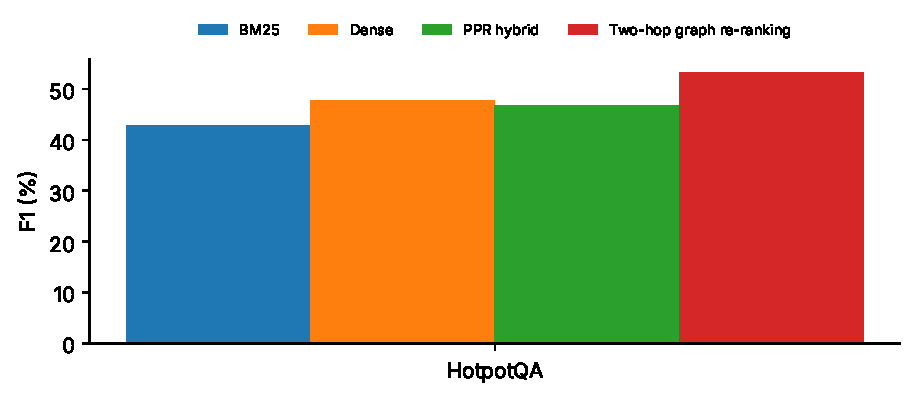
\includegraphics[width=0.78\textwidth]{figs/main.pdf}}{}
\caption{F1 on sample A for the retrievers that were run with the generator (generated by \texttt{make\_tables.py}).}
\label{fig:main}
\end{figure}

\subsection{Efficiency and runtime}\label{sec:cost}
\begin{table}[t]
\centering
\footnotesize
\caption{Retrieval latency per question (ms; mean $\pm$ standard deviation over repeated passes, after warm-up). The cross-encoder rescored the dense top-20.}
\label{tab:timing}
\begin{tabular}{lrrrr}
\toprule
Setting & Dense & Two-hop & Two-hop + gate & CE (dense top-20) \\
\midrule
Cloud CPU: 992 passages & 27 $\pm$ 1 & 162 $\pm$ 5 & 130 $\pm$ 2 & 5725 $\pm$ 37 \\
\bottomrule
\end{tabular}
\end{table}

The laptop run on sample A takes \RSampleABmTwoSec\,s for BM25, \RSampleADenseSec\,s for dense retrieval, \RSampleAHybridSec\,s for the PPR hybrid, \RSampleAHybridTwoSec\,s for the two-hop re-ranker and \ExtHAGateSec\,s with the gate for 1\,000 questions, against \ExtHACESec\,s for the cross-encoder; with the generator included the whole run takes \RHotpotQAHybridTwoSec\,s for the re-ranker, \RHotpotQADenseSec\,s for dense retrieval and \AnsCESec\,s for the cross-encoder. That run was a single pass without warm-up control, so we repeated the measurement. Table~\ref{tab:timing} gives per-question retrieval latency on the two-core cloud CPU after 10 warm-up questions, as the mean and standard deviation of three passes over 90 questions on a 992-passage pool, with batch size one for the question encoder and the cross-encoder scoring 20 pairs per question in one batch. The two-hop re-ranker takes \TmCpukTwo\,$\pm$\,\TmCpukTwoSd\,ms per question against \TmCpukDense\,$\pm$\,\TmCpukDenseSd\,ms for dense retrieval, about \TmCpukSlow{} times more, and \TmCpukGate\,$\pm$\,\TmCpukGateSd\,ms with the gate; the cross-encoder takes \TmCpukCE\,$\pm$\,\TmCpukCESd\,ms. The cost of the cross-encoder relative to the two-hop step is therefore large on this CPU (a factor of about \TmCpukRatio), but the factor depends on hardware, batch size and model, and we do not claim a single ratio. The title-link-only variant needs no extra encoding and is close to dense retrieval in latency. The two-hop cost includes the $m$ extra query encodings, the exhaustive scoring of every expanded query against all passage embeddings and the min--max normalisation over all passages (Section~\ref{sec:method}); it grows linearly with the pool size. Indexing and memory are reported in Table~\ref{tab:scale}: dense encoding dominates indexing time (about \ScaleOneIndexMin{} minutes for 9\,760 passages including graph construction, \ScaleFullIndexMin{} minutes for \ScaleFullPass{} passages), and the process peaks at \ScaleOneRSSgb\,GB and \ScaleFullRSSgb\,GB respectively. These times are for CPU cores and are indicative; the retrieval cost is small next to generation.

\section{Discussion and Limitations}\label{sec:discussion}
\subsection{What the results show}
A graph restricts which passages may be boosted, and a gate keeps the step away from comparison questions. With the settings frozen on HotpotQA, the step raises All@5 on all three datasets, and the control experiments tell us why. The graph-restricted title link accounts for most of the gain on HotpotQA and 2WikiMultiHopQA, where a variant with no query expansion does as well or better; query expansion adds value mainly on MuSiQue, and only when the graph restricts it. The expanded query alone, scored over the whole corpus, gives little. On HotpotQA we detect no significant All@5 difference from a cross-encoder at lower retrieval cost, and the cross-encoder gives no gain on 2WikiMultiHopQA, where candidate coverage of the dense top-20 is low. Personalised PageRank on the same graph did not add anything over BGE. The entity graph needs to be only as good as a capitalised-span extractor. On a common candidate pool the cross-encoder orders passages better than the two-hop score, so the two-hop step contributes mainly candidate discovery, and a cross-encoder on top of its candidates gives the highest All@5 we measured on HotpotQA (Section~\ref{sec:gpu}). On answers, the gated two-hop method is at least as good as TitleLink and better than the cross-encoder on both samples, even where TitleLink retrieves as many supporting passages, so retrieval accuracy alone does not predict answer quality. We caution against reading this as evidence that entity graphs help in general: the benefit we measure is largely a Wikipedia-title effect, and the method follows one bridge, so it did not help on 3-hop and 4-hop MuSiQue questions.

\subsection{What the results do not show}
The data do not show that the method reduces hallucination: the unsupported-answer rate changes by a small amount with an interval that touches zero, and the metric is lexical. They do not show that the method works on a full retrieval corpus, with other encoders, with corpora whose passage titles are not entities, or with larger generators; the corpus-scale test of Section~\ref{sec:controls} enlarges the distractor pool but is still pooled from the development questions. They also do not show that it is better than LLM-built graph retrievers or iterative methods, because the LinearRAG- and SPRIG-style baselines are simplified re-implementations with untuned defaults (the authors' systems were not run), GRiever and iterative methods were not run, and only one cross-encoder was tested.

\subsection{Threats to validity}
\paragraph{Internal validity.} The hyper-parameters and the gate were chosen on the training split, yet sample A had earlier been used to evaluate the PPR variant, and sample B was reused for the extended systems (Section~\ref{sec:evalprot}). The first $\gamma$ sweep hit the edge of its grid and was extended on the training split only. Answers were generated with greedy decoding and a single seed, so generator variance is not measured.
\paragraph{External validity.} The corpora pool the paragraphs of 1\,000 questions each and are far smaller than a Wikipedia index; the gain may shrink with more distractors. The title-link signal is specific to Wikipedia-style titles, and the three datasets are all Wikipedia-based. Answers were generated for HotpotQA only.
\paragraph{Construct validity.} All@5 is necessary but not sufficient for a correct answer. The groundedness proxy compares tokens, not meaning, and cannot detect a contradiction of the evidence. EM and F1 penalise correct answers that are phrased differently. The cross-encoder sees only the top-20, so its All@5 is bounded by the All@20 of its candidate list (Table~\ref{tab:coverage}).
\paragraph{Statistical validity.} The bootstrap treats questions as independent and does not correct for the number of comparisons. The retrieval gains are large relative to their intervals, but the gate effect and the unsupported-answer difference are not.

\subsection{Further limitations and future work}
The title-based gate is a simple rule and trails the oracle gate; a trained question-type classifier is a natural next step. The re-ranker follows a single bridge, so multi-step chains need either an iterated version or a different method. LoRA fine-tuning of the generator \citep{hu2022lora,dettmers2023qlora} was implemented but not evaluated. Official GraphRAG, LightRAG and HippoRAG and iterative LLM-based retrieval are not compared; they may be stronger, at higher cost. Future work also includes larger corpora, other encoders and rerankers, and measuring faithfulness with an entailment-based or claim-level metric \citep{honovich2022true,min2023factscore,es2024ragas} before making any claim about hallucination.

\section{Conclusion}\label{sec:conclusion}
A passage--entity graph built without any LLM call can restrict a second, boosted scoring pass to passages that are linked to the first-hop evidence. On HotpotQA with BGE-small this raises All@5 by about 9 to 12 points on two samples when combined with a question-type gate, and improves the answer F1 of a 1.5B generator. Control experiments show that most of this gain comes from the graph-restricted title link rather than from query expansion: a variant with the title link only is as good or better on HotpotQA and much better on 2WikiMultiHopQA, while the expansion matters on MuSiQue, where the gain is confined to two-hop questions. On HotpotQA we detect no significant All@5 difference from a cross-encoder, which does not show equivalence; the cross-encoder gives no gain on 2WikiMultiHopQA. A cross-encoder on a common candidate pool is the better orderer, and the two-hop step mainly widens the candidate pool; with the same generator the gated two-hop method answers at least as well as TitleLink and better than the cross-encoder on two HotpotQA samples. Without the gate, comparison questions get worse, and a personalised-PageRank walk on the same graph does not help. The study is limited to Wikipedia-based benchmarks with pooled corpora and one encoder, so the results are evidence for a cheap and transparent re-ranking idea whose main ingredient is the title link, not a general claim about graph-based RAG.

\section*{Declaration of generative AI and AI-assisted technologies in the writing process}
During the preparation of this work the authors used Claude (Anthropic) to edit the language of the manuscript and to assist with drafting the text and with writing and debugging the experiment code. After using this tool, the authors reviewed and edited the content as needed and take full responsibility for the content of the published article. The main experiments were run on the authors' laptop and, for the generator-dependent additions, on a GPU server. The control, candidate-coverage, corpus-scale and timing experiments of Sections~\ref{sec:controls} and~\ref{sec:cost} were executed with the released scripts in a cloud container through the same assistant, at the authors' request. All reported numbers are produced by the released scripts from the stored result files.

\section*{Declaration of competing interest}
The authors declare that they have no known competing financial interests or personal relationships that could have appeared to influence the work reported in this paper.

\section*{Funding}
This research received no specific grant from any funding agency in the public, commercial, or not-for-profit sectors.

\section*{Data availability}
HotpotQA \citep{yang2018hotpotqa}, 2WikiMultiHopQA \citep{ho2020twowiki} and MuSiQue \citep{trivedi2022musique} are public datasets. The code, configuration files, tuned hyper-parameters, per-question outputs and the scripts that regenerate every table and figure are available in a public repository at \url{\repourl} and archived on Zenodo (\url{https://doi.org/10.5281/zenodo.23435332}).

\section*{Ethics statement}
The study uses public benchmark data and involves no human participants or personal data.

\printcredits

\bibliographystyle{cas-model2-names}
\bibliography{refs}
\end{document}
